\documentclass[twoside]{book}

% Packages required by doxygen
\usepackage{fixltx2e}
\usepackage{calc}
\usepackage{doxygen}
\usepackage{graphicx}
\usepackage[utf8]{inputenc}
\usepackage{makeidx}
\usepackage{multicol}
\usepackage{multirow}
\PassOptionsToPackage{warn}{textcomp}
\usepackage{textcomp}
\usepackage[nointegrals]{wasysym}
\usepackage[table]{xcolor}

% Font selection
\usepackage[T1]{fontenc}
\usepackage{mathptmx}
\usepackage[scaled=.90]{helvet}
\usepackage{courier}
\usepackage{amssymb}
\usepackage{sectsty}
\renewcommand{\familydefault}{\sfdefault}
\allsectionsfont{%
  \fontseries{bc}\selectfont%
  \color{darkgray}%
}
\renewcommand{\DoxyLabelFont}{%
  \fontseries{bc}\selectfont%
  \color{darkgray}%
}
\newcommand{\+}{\discretionary{\mbox{\scriptsize$\hookleftarrow$}}{}{}}

% Page & text layout
\usepackage{geometry}
\geometry{%
  a4paper,%
  top=2.5cm,%
  bottom=2.5cm,%
  left=2.5cm,%
  right=2.5cm%
}
\tolerance=750
\hfuzz=15pt
\hbadness=750
\setlength{\emergencystretch}{15pt}
\setlength{\parindent}{0cm}
\setlength{\parskip}{0.2cm}
\makeatletter
\renewcommand{\paragraph}{%
  \@startsection{paragraph}{4}{0ex}{-1.0ex}{1.0ex}{%
    \normalfont\normalsize\bfseries\SS@parafont%
  }%
}
\renewcommand{\subparagraph}{%
  \@startsection{subparagraph}{5}{0ex}{-1.0ex}{1.0ex}{%
    \normalfont\normalsize\bfseries\SS@subparafont%
  }%
}
\makeatother

% Headers & footers
\usepackage{fancyhdr}
\pagestyle{fancyplain}
\fancyhead[LE]{\fancyplain{}{\bfseries\thepage}}
\fancyhead[CE]{\fancyplain{}{}}
\fancyhead[RE]{\fancyplain{}{\bfseries\leftmark}}
\fancyhead[LO]{\fancyplain{}{\bfseries\rightmark}}
\fancyhead[CO]{\fancyplain{}{}}
\fancyhead[RO]{\fancyplain{}{\bfseries\thepage}}
\fancyfoot[LE]{\fancyplain{}{}}
\fancyfoot[CE]{\fancyplain{}{}}
\fancyfoot[RE]{\fancyplain{}{\bfseries\scriptsize Generated on Fri Sep 4 2015 08\+:01\+:31 for Módulo de reconocimiento by Doxygen }}
\fancyfoot[LO]{\fancyplain{}{\bfseries\scriptsize Generated on Fri Sep 4 2015 08\+:01\+:31 for Módulo de reconocimiento by Doxygen }}
\fancyfoot[CO]{\fancyplain{}{}}
\fancyfoot[RO]{\fancyplain{}{}}
\renewcommand{\footrulewidth}{0.4pt}
\renewcommand{\chaptermark}[1]{%
  \markboth{#1}{}%
}
\renewcommand{\sectionmark}[1]{%
  \markright{\thesection\ #1}%
}

% Indices & bibliography
\usepackage{natbib}
\usepackage[titles]{tocloft}
\setcounter{tocdepth}{3}
\setcounter{secnumdepth}{5}
\makeindex

% Hyperlinks (required, but should be loaded last)
\usepackage{ifpdf}
\ifpdf
  \usepackage[pdftex,pagebackref=true]{hyperref}
\else
  \usepackage[ps2pdf,pagebackref=true]{hyperref}
\fi
\hypersetup{%
  colorlinks=true,%
  linkcolor=blue,%
  citecolor=blue,%
  unicode%
}

% Custom commands
\newcommand{\clearemptydoublepage}{%
  \newpage{\pagestyle{empty}\cleardoublepage}%
}


%===== C O N T E N T S =====

\begin{document}

% Titlepage & ToC
\hypersetup{pageanchor=false,
             bookmarks=true,
             bookmarksnumbered=true,
             pdfencoding=unicode
            }
\pagenumbering{roman}
\begin{titlepage}
\vspace*{7cm}
\begin{center}%
{\Large Módulo de reconocimiento }\\
\vspace*{1cm}
{\large Generated by Doxygen 1.8.8}\\
\vspace*{0.5cm}
{\small Fri Sep 4 2015 08:01:31}\\
\end{center}
\end{titlepage}
\clearemptydoublepage
\tableofcontents
\clearemptydoublepage
\pagenumbering{arabic}
\hypersetup{pageanchor=true}

%--- Begin generated contents ---
\chapter{Módulo de reconocimiento}
\label{index}\hypertarget{index}{}Este documento recoge la documentación asocidada al módulo de reconocimiento 
\chapter{Hierarchical Index}
\section{Class Hierarchy}
This inheritance list is sorted roughly, but not completely, alphabetically\+:\begin{DoxyCompactList}
\item \contentsline{section}{Angle}{\pageref{class_angle}}{}
\item \contentsline{section}{Binarization}{\pageref{class_binarization}}{}
\item \contentsline{section}{Filter}{\pageref{class_filter}}{}
\item \contentsline{section}{Frequency}{\pageref{class_frequency}}{}
\item \contentsline{section}{Matching}{\pageref{class_matching}}{}
\item \contentsline{section}{Math\+Operation}{\pageref{class_math_operation}}{}
\item \contentsline{section}{Minutia}{\pageref{class_minutia}}{}
\item \contentsline{section}{Minutia\+Extractor}{\pageref{class_minutia_extractor}}{}
\item \contentsline{section}{Normalize}{\pageref{class_normalize}}{}
\item \contentsline{section}{Orientation}{\pageref{class_orientation}}{}
\item Q\+Main\+Window\begin{DoxyCompactList}
\item \contentsline{section}{Main\+Window}{\pageref{class_main_window}}{}
\end{DoxyCompactList}
\item Q\+Object\begin{DoxyCompactList}
\item \contentsline{section}{Process\+Fingerprint}{\pageref{class_process_fingerprint}}{}
\end{DoxyCompactList}
\item Q\+Widget\begin{DoxyCompactList}
\item \contentsline{section}{Fingerprint\+Loader}{\pageref{class_fingerprint_loader}}{}
\end{DoxyCompactList}
\item \contentsline{section}{Segmentation}{\pageref{class_segmentation}}{}
\item \contentsline{section}{Thinning}{\pageref{class_thinning}}{}
\end{DoxyCompactList}

\chapter{Class Index}
\section{Class List}
Here are the classes, structs, unions and interfaces with brief descriptions\+:\begin{DoxyCompactList}
\item\contentsline{section}{\hyperlink{class_angle}{Angle} \\*Clase encargada del cálculo y transformación de ángulos }{\pageref{class_angle}}{}
\item\contentsline{section}{\hyperlink{class_binarization}{Binarization} \\*Clase que recoge la funcionalidad encargada de realizar la binarizacion de la imagen }{\pageref{class_binarization}}{}
\item\contentsline{section}{\hyperlink{class_filter}{Filter} \\*Clase que recoge la funcionalidad encargada de realizar los distintos filtros sobre la imagen }{\pageref{class_filter}}{}
\item\contentsline{section}{\hyperlink{class_fingerprint_loader}{Fingerprint\+Loader} \\*Clase encargada de la carga de las imagenes de las huellas dactilares }{\pageref{class_fingerprint_loader}}{}
\item\contentsline{section}{\hyperlink{class_frequency}{Frequency} \\*Clase que recoge la funcionalidad encargada de realizar el calculo de la frecuencia de la imagen }{\pageref{class_frequency}}{}
\item\contentsline{section}{\hyperlink{class_main_window}{Main\+Window} \\*Clase encargada del control de la interfaz }{\pageref{class_main_window}}{}
\item\contentsline{section}{\hyperlink{class_matching}{Matching} \\*Clase que recoge la funcionalidad encargada de realizar el proceso de matchin }{\pageref{class_matching}}{}
\item\contentsline{section}{\hyperlink{class_math_operation}{Math\+Operation} \\*Clase en la que se recogen las funciones matematicas necesitadas por el modulo }{\pageref{class_math_operation}}{}
\item\contentsline{section}{\hyperlink{class_minutia}{Minutia} \\*Clase que va a contener las caracteristicas de la minucias }{\pageref{class_minutia}}{}
\item\contentsline{section}{\hyperlink{class_minutia_extractor}{Minutia\+Extractor} \\*Clase que recoge la funcionalidad encargada de realizar la extraccion de minucias de la imagen }{\pageref{class_minutia_extractor}}{}
\item\contentsline{section}{\hyperlink{class_normalize}{Normalize} \\*Clase que recoge la funcionalidad encargada de realizar la normalizacion de la imagen }{\pageref{class_normalize}}{}
\item\contentsline{section}{\hyperlink{class_orientation}{Orientation} \\*Clase que recoge la funcionalidad encargada de realizar la orientacion de la imagen }{\pageref{class_orientation}}{}
\item\contentsline{section}{\hyperlink{class_process_fingerprint}{Process\+Fingerprint} \\*Clase que recoge la funcionalidad encargada de encamsular el procesamiento de la imagen }{\pageref{class_process_fingerprint}}{}
\item\contentsline{section}{\hyperlink{class_segmentation}{Segmentation} \\*Clase que recoge la funcionalidad encargada de realizar la segmentacion de la imagen }{\pageref{class_segmentation}}{}
\item\contentsline{section}{\hyperlink{class_thinning}{Thinning} \\*Clase que recoge la funcionalidad encargada de realizar el adelgazamiento de la imagen }{\pageref{class_thinning}}{}
\end{DoxyCompactList}

\chapter{Class Documentation}
\hypertarget{class_angle}{\section{Angle Class Reference}
\label{class_angle}\index{Angle@{Angle}}
}


The \hyperlink{class_angle}{Angle} class Clase encargada del cálculo y transformación de ángulos.  




{\ttfamily \#include $<$angle.\+h$>$}

\subsection*{Public Member Functions}
\begin{DoxyCompactItemize}
\item 
\hypertarget{class_angle_aca3c6e1519b40835d31736430ca082a9}{\hyperlink{class_angle_aca3c6e1519b40835d31736430ca082a9}{Angle} ()}\label{class_angle_aca3c6e1519b40835d31736430ca082a9}

\begin{DoxyCompactList}\small\item\em \hyperlink{class_angle}{Angle} Constructor vacío. \end{DoxyCompactList}\end{DoxyCompactItemize}
\subsection*{Static Public Member Functions}
\begin{DoxyCompactItemize}
\item 
static double \hyperlink{class_angle_ab883e3d7040fd7cfcf0e90da2cbe84ad}{compute\+Angle\+In\+Radians} (float d\+Y, float d\+X)
\begin{DoxyCompactList}\small\item\em compute\+Angle\+In\+Radians Método que calcula el angulo en radianes dado a partir de dos valores utilizando la arcotangente \end{DoxyCompactList}\item 
static double \hyperlink{class_angle_a5dfc4cbb910399852dae886aa0d032e6}{to\+Radians} (float deg)
\begin{DoxyCompactList}\small\item\em to\+Radians Metodo que realiza la transformacion de un angulo de grados a radianes \end{DoxyCompactList}\item 
static double \hyperlink{class_angle_ab8e04a32bd7ca82f75621000e2ba8547}{to\+Degrees} (float rad)
\begin{DoxyCompactList}\small\item\em to\+Degrees Metodo que realiza la transformacion de un angulo de radianes a grados \end{DoxyCompactList}\item 
static double \hyperlink{class_angle_ae1eaf7179e1986c65820bc0f9aa5e45b}{difference\+Pi} (double angle\+A, double angle\+B)
\begin{DoxyCompactList}\small\item\em difference\+Pi Metodo que calcula la menor diferencia entre dos angulos \end{DoxyCompactList}\end{DoxyCompactItemize}


\subsection{Detailed Description}
The \hyperlink{class_angle}{Angle} class Clase encargada del cálculo y transformación de ángulos. 

\subsection{Member Function Documentation}
\hypertarget{class_angle_ab883e3d7040fd7cfcf0e90da2cbe84ad}{\index{Angle@{Angle}!compute\+Angle\+In\+Radians@{compute\+Angle\+In\+Radians}}
\index{compute\+Angle\+In\+Radians@{compute\+Angle\+In\+Radians}!Angle@{Angle}}
\subsubsection[{compute\+Angle\+In\+Radians}]{\setlength{\rightskip}{0pt plus 5cm}double Angle\+::compute\+Angle\+In\+Radians (
\begin{DoxyParamCaption}
\item[{float}]{d\+Y, }
\item[{float}]{d\+X}
\end{DoxyParamCaption}
)\hspace{0.3cm}{\ttfamily [static]}}}\label{class_angle_ab883e3d7040fd7cfcf0e90da2cbe84ad}


compute\+Angle\+In\+Radians Método que calcula el angulo en radianes dado a partir de dos valores utilizando la arcotangente 


\begin{DoxyParams}{Parameters}
{\em d\+X} & Float en el eje x \\
\hline
{\em d\+Y} & Float en el eje y \\
\hline
\end{DoxyParams}
\begin{DoxyReturn}{Returns}
Double que contiene el angulo en radianes 
\end{DoxyReturn}
\hypertarget{class_angle_ae1eaf7179e1986c65820bc0f9aa5e45b}{\index{Angle@{Angle}!difference\+Pi@{difference\+Pi}}
\index{difference\+Pi@{difference\+Pi}!Angle@{Angle}}
\subsubsection[{difference\+Pi}]{\setlength{\rightskip}{0pt plus 5cm}double Angle\+::difference\+Pi (
\begin{DoxyParamCaption}
\item[{double}]{angle\+A, }
\item[{double}]{angle\+B}
\end{DoxyParamCaption}
)\hspace{0.3cm}{\ttfamily [static]}}}\label{class_angle_ae1eaf7179e1986c65820bc0f9aa5e45b}


difference\+Pi Metodo que calcula la menor diferencia entre dos angulos 


\begin{DoxyParams}{Parameters}
{\em alpha} & Angulo 1 \\
\hline
{\em beta} & Angulo 2 \\
\hline
\end{DoxyParams}
\begin{DoxyReturn}{Returns}
Diferencia entre angulos 
\end{DoxyReturn}
\hypertarget{class_angle_ab8e04a32bd7ca82f75621000e2ba8547}{\index{Angle@{Angle}!to\+Degrees@{to\+Degrees}}
\index{to\+Degrees@{to\+Degrees}!Angle@{Angle}}
\subsubsection[{to\+Degrees}]{\setlength{\rightskip}{0pt plus 5cm}double Angle\+::to\+Degrees (
\begin{DoxyParamCaption}
\item[{float}]{rad}
\end{DoxyParamCaption}
)\hspace{0.3cm}{\ttfamily [static]}}}\label{class_angle_ab8e04a32bd7ca82f75621000e2ba8547}


to\+Degrees Metodo que realiza la transformacion de un angulo de radianes a grados 


\begin{DoxyParams}{Parameters}
{\em rad} & Angulo en radianes \\
\hline
\end{DoxyParams}
\begin{DoxyReturn}{Returns}
Double que contiene el angulo en grados 
\end{DoxyReturn}
\hypertarget{class_angle_a5dfc4cbb910399852dae886aa0d032e6}{\index{Angle@{Angle}!to\+Radians@{to\+Radians}}
\index{to\+Radians@{to\+Radians}!Angle@{Angle}}
\subsubsection[{to\+Radians}]{\setlength{\rightskip}{0pt plus 5cm}double Angle\+::to\+Radians (
\begin{DoxyParamCaption}
\item[{float}]{deg}
\end{DoxyParamCaption}
)\hspace{0.3cm}{\ttfamily [static]}}}\label{class_angle_a5dfc4cbb910399852dae886aa0d032e6}


to\+Radians Metodo que realiza la transformacion de un angulo de grados a radianes 


\begin{DoxyParams}{Parameters}
{\em deg} & Angulo en grados \\
\hline
\end{DoxyParams}
\begin{DoxyReturn}{Returns}
Double que contiene el angulo en radianes 
\end{DoxyReturn}


The documentation for this class was generated from the following files\+:\begin{DoxyCompactItemize}
\item 
angle.\+h\item 
angle.\+cpp\end{DoxyCompactItemize}

\hypertarget{class_binarization}{\section{Binarization Class Reference}
\label{class_binarization}\index{Binarization@{Binarization}}
}


The \hyperlink{class_binarization}{Binarization} class Clase que recoge la funcionalidad encargada de realizar la binarizacion de la imagen.  




{\ttfamily \#include $<$binarization.\+h$>$}

\subsection*{Public Member Functions}
\begin{DoxyCompactItemize}
\item 
\hypertarget{class_binarization_a2227910fd9f1600f0f31c65285a8fc08}{\hyperlink{class_binarization_a2227910fd9f1600f0f31c65285a8fc08}{Binarization} ()}\label{class_binarization_a2227910fd9f1600f0f31c65285a8fc08}

\begin{DoxyCompactList}\small\item\em \hyperlink{class_binarization}{Binarization}. \end{DoxyCompactList}\item 
\hyperlink{class_binarization_a8ee0e3bd1fbc4347b1e34f9409970bb6}{Binarization} (int h, int w)
\begin{DoxyCompactList}\small\item\em \hyperlink{class_binarization}{Binarization}. \end{DoxyCompactList}\item 
void \hyperlink{class_binarization_a7cf4b278e99a38c12da399e33cc690cf}{binarize} (cv\+::\+Mat \&src, cv\+::\+Mat \&oi\+Matrix, cv\+::\+Mat \&segmented\+Matrix, int threshold, int block\+Size)
\begin{DoxyCompactList}\small\item\em binarize \end{DoxyCompactList}\end{DoxyCompactItemize}
\subsection*{Public Attributes}
\begin{DoxyCompactItemize}
\item 
\hypertarget{class_binarization_a4e1c66ac5f6ded0bfd845039025483ed}{cv\+::\+Mat \hyperlink{class_binarization_a4e1c66ac5f6ded0bfd845039025483ed}{bin\+Matrix}}\label{class_binarization_a4e1c66ac5f6ded0bfd845039025483ed}

\begin{DoxyCompactList}\small\item\em bin\+Matrix cv\+::\+Mat que contiene la imagen binarizada \end{DoxyCompactList}\end{DoxyCompactItemize}


\subsection{Detailed Description}
The \hyperlink{class_binarization}{Binarization} class Clase que recoge la funcionalidad encargada de realizar la binarizacion de la imagen. 

\subsection{Constructor \& Destructor Documentation}
\hypertarget{class_binarization_a8ee0e3bd1fbc4347b1e34f9409970bb6}{\index{Binarization@{Binarization}!Binarization@{Binarization}}
\index{Binarization@{Binarization}!Binarization@{Binarization}}
\subsubsection[{Binarization}]{\setlength{\rightskip}{0pt plus 5cm}Binarization\+::\+Binarization (
\begin{DoxyParamCaption}
\item[{int}]{h, }
\item[{int}]{w}
\end{DoxyParamCaption}
)}}\label{class_binarization_a8ee0e3bd1fbc4347b1e34f9409970bb6}


\hyperlink{class_binarization}{Binarization}. 


\begin{DoxyParams}{Parameters}
{\em h} & Entero que especifica el número de columnas del objeto cv\+::\+Mat que va a contoner la imagen binarizada \\
\hline
{\em w} & Entero que especifica el número de columnas del objeto cv\+::\+Mat que va a contoner la imagen binarizada \\
\hline
\end{DoxyParams}


\subsection{Member Function Documentation}
\hypertarget{class_binarization_a7cf4b278e99a38c12da399e33cc690cf}{\index{Binarization@{Binarization}!binarize@{binarize}}
\index{binarize@{binarize}!Binarization@{Binarization}}
\subsubsection[{binarize}]{\setlength{\rightskip}{0pt plus 5cm}void Binarization\+::binarize (
\begin{DoxyParamCaption}
\item[{cv\+::\+Mat \&}]{src, }
\item[{cv\+::\+Mat \&}]{oi\+Matrix, }
\item[{cv\+::\+Mat \&}]{segmented\+Matrix, }
\item[{int}]{threshold, }
\item[{int}]{block\+Size}
\end{DoxyParamCaption}
)}}\label{class_binarization_a7cf4b278e99a38c12da399e33cc690cf}


binarize 


\begin{DoxyParams}{Parameters}
{\em src} & cv\+::\+Mat que contiene la imagen original que se va a binarizar \\
\hline
{\em oi\+Matrix} & cv\+::\+Mat que contiene la orientacion de la imagen que se va a binarizar \\
\hline
{\em segmented\+Matrix} & cv\+::\+Mat que contiene la mascara de segmentación de la imagen normalizada \\
\hline
{\em threshold} & Entero que indica el valor threshold utilizado para realizar la binarizacion \\
\hline
{\em block\+Size} & Entero que indica el tamaño del bloque utilizado en la orientacion \\
\hline
\end{DoxyParams}
Todos los valores que sean menores que el threshold y esten dentro de la mascara se ponen a 0

Si el bloque en el que se encuentran los pixeles es nulo, se ponen a 255

The documentation for this class was generated from the following files\+:\begin{DoxyCompactItemize}
\item 
binarization.\+h\item 
binarization.\+cpp\end{DoxyCompactItemize}

\hypertarget{class_filter}{\section{Filter Class Reference}
\label{class_filter}\index{Filter@{Filter}}
}


The \hyperlink{class_filter}{Filter} class Clase que recoge la funcionalidad encargada de realizar los distintos filtros sobre la imagen.  




{\ttfamily \#include $<$filter.\+h$>$}

\subsection*{Public Member Functions}
\begin{DoxyCompactItemize}
\item 
\hypertarget{class_filter_ad15994c30d497afd567a6445446a249e}{\hyperlink{class_filter_ad15994c30d497afd567a6445446a249e}{Filter} ()}\label{class_filter_ad15994c30d497afd567a6445446a249e}

\begin{DoxyCompactList}\small\item\em \hyperlink{class_filter}{Filter} Constructor vacio. \end{DoxyCompactList}\item 
void \hyperlink{class_filter_a22cd4f0258d34426a3a3155a12d1c574}{apply\+Gabor\+Filter} (cv\+::\+Mat \&src, cv\+::\+Mat \&oi\+Matrix, cv\+::\+Mat \&freq\+Matrix, cv\+::\+Mat \&gabor\+Matrix, int block\+Size)
\begin{DoxyCompactList}\small\item\em apply\+Gabor\+Filter Metodo utilizado para la aplicación de los filtros de Gabor sobre una imagen \end{DoxyCompactList}\item 
void \hyperlink{class_filter_a1c28fce1c31afe8e44c5c059593e686b}{apply\+Gabor\+Filter\+To\+Chunk} (cv\+::\+Mat \&src, cv\+::\+Mat \&oi\+Matrix, cv\+::\+Mat \&freq\+Matrix, cv\+::\+Mat \&gabor\+Matrix, int min, int max, int block\+Size)
\begin{DoxyCompactList}\small\item\em apply\+Gabor\+Filter\+To\+Chunk Metodo utilizado para la aplicación de los filtros de Gabor sobre una imagen \end{DoxyCompactList}\item 
cv\+::\+Mat \hyperlink{class_filter_a0d8a2b258d04ed38be4e37cc7a5a4d76}{apply\+Sobel\+Filter\+X} (cv\+::\+Mat \&src)
\begin{DoxyCompactList}\small\item\em apply\+Sobel\+Filter\+X \end{DoxyCompactList}\item 
cv\+::\+Mat \hyperlink{class_filter_a72c5cd12e966515a3683ae61a16fa26d}{apply\+Sobel\+Filter\+Y} (cv\+::\+Mat \&src)
\begin{DoxyCompactList}\small\item\em apply\+Sobel\+Filter\+Y \end{DoxyCompactList}\end{DoxyCompactItemize}


\subsection{Detailed Description}
The \hyperlink{class_filter}{Filter} class Clase que recoge la funcionalidad encargada de realizar los distintos filtros sobre la imagen. 

\subsection{Member Function Documentation}
\hypertarget{class_filter_a22cd4f0258d34426a3a3155a12d1c574}{\index{Filter@{Filter}!apply\+Gabor\+Filter@{apply\+Gabor\+Filter}}
\index{apply\+Gabor\+Filter@{apply\+Gabor\+Filter}!Filter@{Filter}}
\subsubsection[{apply\+Gabor\+Filter}]{\setlength{\rightskip}{0pt plus 5cm}void Filter\+::apply\+Gabor\+Filter (
\begin{DoxyParamCaption}
\item[{cv\+::\+Mat \&}]{src, }
\item[{cv\+::\+Mat \&}]{oi\+Matrix, }
\item[{cv\+::\+Mat \&}]{freq\+Matrix, }
\item[{cv\+::\+Mat \&}]{gabor\+Matrix, }
\item[{int}]{block\+Size}
\end{DoxyParamCaption}
)}}\label{class_filter_a22cd4f0258d34426a3a3155a12d1c574}


apply\+Gabor\+Filter Metodo utilizado para la aplicación de los filtros de Gabor sobre una imagen 


\begin{DoxyParams}{Parameters}
{\em src} & cv\+::\+Mat que contiene la imagen original que se va a filtrar \\
\hline
{\em oi\+Matrix} & cv\+::\+Mat que contiene la orientacion de la imagen que se va a filtrar \\
\hline
{\em freq\+Matrix} & cv\+::\+Mat que contiene la frecuencia de la imagen que se va a filtrar \\
\hline
{\em gabor\+Matrix} & cv\+::\+Mat que va a contener la imagen filtrada \\
\hline
{\em block\+Size} & cv\+:\+: Tamaño de bloque que se va a usar en el proceso de filtrado \\
\hline
\end{DoxyParams}
\hypertarget{class_filter_a1c28fce1c31afe8e44c5c059593e686b}{\index{Filter@{Filter}!apply\+Gabor\+Filter\+To\+Chunk@{apply\+Gabor\+Filter\+To\+Chunk}}
\index{apply\+Gabor\+Filter\+To\+Chunk@{apply\+Gabor\+Filter\+To\+Chunk}!Filter@{Filter}}
\subsubsection[{apply\+Gabor\+Filter\+To\+Chunk}]{\setlength{\rightskip}{0pt plus 5cm}void Filter\+::apply\+Gabor\+Filter\+To\+Chunk (
\begin{DoxyParamCaption}
\item[{cv\+::\+Mat \&}]{src, }
\item[{cv\+::\+Mat \&}]{oi\+Matrix, }
\item[{cv\+::\+Mat \&}]{freq\+Matrix, }
\item[{cv\+::\+Mat \&}]{gabor\+Matrix, }
\item[{int}]{min, }
\item[{int}]{max, }
\item[{int}]{block\+Size}
\end{DoxyParamCaption}
)}}\label{class_filter_a1c28fce1c31afe8e44c5c059593e686b}


apply\+Gabor\+Filter\+To\+Chunk Metodo utilizado para la aplicación de los filtros de Gabor sobre una imagen 


\begin{DoxyParams}{Parameters}
{\em src} & cv\+::\+Mat que contiene la imagen original que se va a filtrar \\
\hline
{\em oi\+Matrix} & cv\+::\+Mat que contiene la orientacion de la imagen que se va a filtrar \\
\hline
{\em freq\+Matrix} & cv\+::\+Mat que contiene la frecuencia de la imagen que se va a filtrar \\
\hline
{\em gabor\+Matrix} & cv\+::\+Mat que va a contener la imagen filtrada \\
\hline
{\em min} & \\
\hline
{\em max} & \\
\hline
{\em block\+Size} & cv\+:\+: Tamaño de bloque que se va a usar en el proceso de filtrado \\
\hline
\end{DoxyParams}
\hypertarget{class_filter_a0d8a2b258d04ed38be4e37cc7a5a4d76}{\index{Filter@{Filter}!apply\+Sobel\+Filter\+X@{apply\+Sobel\+Filter\+X}}
\index{apply\+Sobel\+Filter\+X@{apply\+Sobel\+Filter\+X}!Filter@{Filter}}
\subsubsection[{apply\+Sobel\+Filter\+X}]{\setlength{\rightskip}{0pt plus 5cm}cv\+::\+Mat Filter\+::apply\+Sobel\+Filter\+X (
\begin{DoxyParamCaption}
\item[{cv\+::\+Mat \&}]{src}
\end{DoxyParamCaption}
)}}\label{class_filter_a0d8a2b258d04ed38be4e37cc7a5a4d76}


apply\+Sobel\+Filter\+X 


\begin{DoxyParams}{Parameters}
{\em src} & cv\+::\+Mat que contiene la imagen original que se va a filtrar \\
\hline
\end{DoxyParams}
\begin{DoxyReturn}{Returns}
cv\+:Mat que va a contener la imagen filtrada 
\end{DoxyReturn}
\hypertarget{class_filter_a72c5cd12e966515a3683ae61a16fa26d}{\index{Filter@{Filter}!apply\+Sobel\+Filter\+Y@{apply\+Sobel\+Filter\+Y}}
\index{apply\+Sobel\+Filter\+Y@{apply\+Sobel\+Filter\+Y}!Filter@{Filter}}
\subsubsection[{apply\+Sobel\+Filter\+Y}]{\setlength{\rightskip}{0pt plus 5cm}cv\+::\+Mat Filter\+::apply\+Sobel\+Filter\+Y (
\begin{DoxyParamCaption}
\item[{cv\+::\+Mat \&}]{src}
\end{DoxyParamCaption}
)}}\label{class_filter_a72c5cd12e966515a3683ae61a16fa26d}


apply\+Sobel\+Filter\+Y 


\begin{DoxyParams}{Parameters}
{\em src} & cv\+::\+Mat que contiene la imagen original que se va a filtrar \\
\hline
\end{DoxyParams}
\begin{DoxyReturn}{Returns}
cv\+:Mat que va a contener la imagen filtrada 
\end{DoxyReturn}


The documentation for this class was generated from the following files\+:\begin{DoxyCompactItemize}
\item 
filter.\+h\item 
filter.\+cpp\end{DoxyCompactItemize}

\hypertarget{class_fingerprint_loader}{\section{Fingerprint\+Loader Class Reference}
\label{class_fingerprint_loader}\index{Fingerprint\+Loader@{Fingerprint\+Loader}}
}


The \hyperlink{class_fingerprint_loader}{Fingerprint\+Loader} class Clase encargada de la carga de las imagenes de las huellas dactilares.  




{\ttfamily \#include $<$fingerprintloader.\+h$>$}

Inheritance diagram for Fingerprint\+Loader\+:\begin{figure}[H]
\begin{center}
\leavevmode
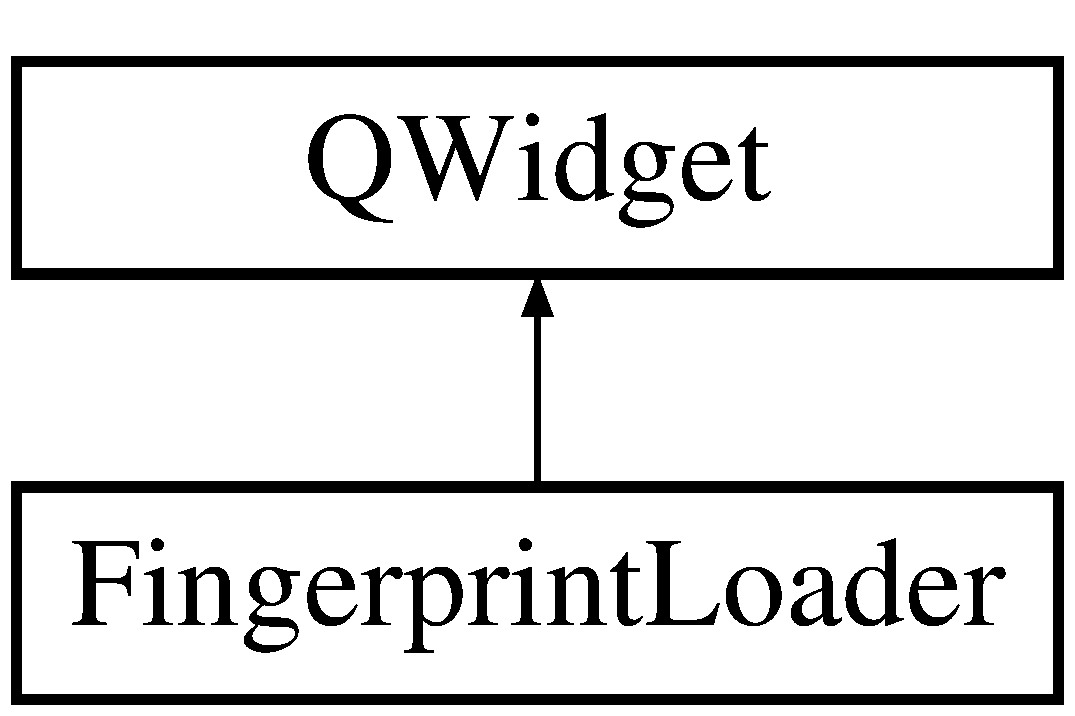
\includegraphics[height=2.000000cm]{class_fingerprint_loader}
\end{center}
\end{figure}
\subsection*{Public Member Functions}
\begin{DoxyCompactItemize}
\item 
\hyperlink{class_fingerprint_loader_a65cbd2252d3f732c934cd9812657a91c}{Fingerprint\+Loader} (Q\+Widget $\ast$parent=0)
\begin{DoxyCompactList}\small\item\em \hyperlink{class_fingerprint_loader}{Fingerprint\+Loader} Constructor. \end{DoxyCompactList}\item 
cv\+::\+Mat \hyperlink{class_fingerprint_loader_a39d7b63a1c6c6f6bd49310414f684cd1}{load\+From\+File} ()
\begin{DoxyCompactList}\small\item\em load\+From\+File Metodo que se encarga de cargar la huella dactilar desde un archivo \end{DoxyCompactList}\item 
cv\+::\+Mat \hyperlink{class_fingerprint_loader_a55a78ad38771cbec91d967a0a59c8ac3}{load\+From\+Scanner} ()
\begin{DoxyCompactList}\small\item\em load\+From\+Scanner Metodo que se encarga de cargar la huella dactilar desde el escaner \end{DoxyCompactList}\end{DoxyCompactItemize}


\subsection{Detailed Description}
The \hyperlink{class_fingerprint_loader}{Fingerprint\+Loader} class Clase encargada de la carga de las imagenes de las huellas dactilares. 

\subsection{Constructor \& Destructor Documentation}
\hypertarget{class_fingerprint_loader_a65cbd2252d3f732c934cd9812657a91c}{\index{Fingerprint\+Loader@{Fingerprint\+Loader}!Fingerprint\+Loader@{Fingerprint\+Loader}}
\index{Fingerprint\+Loader@{Fingerprint\+Loader}!Fingerprint\+Loader@{Fingerprint\+Loader}}
\subsubsection[{Fingerprint\+Loader}]{\setlength{\rightskip}{0pt plus 5cm}Fingerprint\+Loader\+::\+Fingerprint\+Loader (
\begin{DoxyParamCaption}
\item[{Q\+Widget $\ast$}]{parent = {\ttfamily 0}}
\end{DoxyParamCaption}
)\hspace{0.3cm}{\ttfamily [explicit]}}}\label{class_fingerprint_loader_a65cbd2252d3f732c934cd9812657a91c}


\hyperlink{class_fingerprint_loader}{Fingerprint\+Loader} Constructor. 


\begin{DoxyParams}{Parameters}
{\em parent} & Padre de la clase \\
\hline
\end{DoxyParams}


\subsection{Member Function Documentation}
\hypertarget{class_fingerprint_loader_a39d7b63a1c6c6f6bd49310414f684cd1}{\index{Fingerprint\+Loader@{Fingerprint\+Loader}!load\+From\+File@{load\+From\+File}}
\index{load\+From\+File@{load\+From\+File}!Fingerprint\+Loader@{Fingerprint\+Loader}}
\subsubsection[{load\+From\+File}]{\setlength{\rightskip}{0pt plus 5cm}cv\+::\+Mat Fingerprint\+Loader\+::load\+From\+File (
\begin{DoxyParamCaption}
{}
\end{DoxyParamCaption}
)}}\label{class_fingerprint_loader_a39d7b63a1c6c6f6bd49310414f684cd1}


load\+From\+File Metodo que se encarga de cargar la huella dactilar desde un archivo 

\begin{DoxyReturn}{Returns}
cv\+::\+Mat que contiene la imagen leida 
\end{DoxyReturn}
\hypertarget{class_fingerprint_loader_a55a78ad38771cbec91d967a0a59c8ac3}{\index{Fingerprint\+Loader@{Fingerprint\+Loader}!load\+From\+Scanner@{load\+From\+Scanner}}
\index{load\+From\+Scanner@{load\+From\+Scanner}!Fingerprint\+Loader@{Fingerprint\+Loader}}
\subsubsection[{load\+From\+Scanner}]{\setlength{\rightskip}{0pt plus 5cm}cv\+::\+Mat Fingerprint\+Loader\+::load\+From\+Scanner (
\begin{DoxyParamCaption}
{}
\end{DoxyParamCaption}
)}}\label{class_fingerprint_loader_a55a78ad38771cbec91d967a0a59c8ac3}


load\+From\+Scanner Metodo que se encarga de cargar la huella dactilar desde el escaner 

\begin{DoxyReturn}{Returns}
cv\+::\+Mat que contiene la imagen leida 
\end{DoxyReturn}


The documentation for this class was generated from the following files\+:\begin{DoxyCompactItemize}
\item 
fingerprintloader.\+h\item 
fingerprintloader.\+cpp\end{DoxyCompactItemize}

\hypertarget{class_frequency}{\section{Frequency Class Reference}
\label{class_frequency}\index{Frequency@{Frequency}}
}


The \hyperlink{class_frequency}{Frequency} class Clase que recoge la funcionalidad encargada de realizar el calculo de la frecuencia de la imagen.  




{\ttfamily \#include $<$frequency.\+h$>$}

\subsection*{Public Member Functions}
\begin{DoxyCompactItemize}
\item 
\hypertarget{class_frequency_a640e818df1d6e68f508dc21d305a7d22}{\hyperlink{class_frequency_a640e818df1d6e68f508dc21d305a7d22}{Frequency} ()}\label{class_frequency_a640e818df1d6e68f508dc21d305a7d22}

\begin{DoxyCompactList}\small\item\em \hyperlink{class_frequency}{Frequency} Constructor vacio. \end{DoxyCompactList}\item 
void \hyperlink{class_frequency_a073d778d1e37d4d83a9f52c1ba296b05}{calculate\+Frequency\+Block} (cv\+::\+Mat \&src, cv\+::\+Mat \&oi\+Matrix, int block\+Size)
\begin{DoxyCompactList}\small\item\em calculate\+Frequency\+Block Metodo que va a realizar el calculo de la frecuencia de la imagen recibida \end{DoxyCompactList}\end{DoxyCompactItemize}
\subsection*{Public Attributes}
\begin{DoxyCompactItemize}
\item 
\hypertarget{class_frequency_aa6fb6a46b73f44c471ee929d10f7d8d4}{cv\+::\+Mat \hyperlink{class_frequency_aa6fb6a46b73f44c471ee929d10f7d8d4}{freq\+Matrix}}\label{class_frequency_aa6fb6a46b73f44c471ee929d10f7d8d4}

\begin{DoxyCompactList}\small\item\em freq\+Matrix cv\+::\+Mat que contiene frecuencia de la imagen \end{DoxyCompactList}\end{DoxyCompactItemize}


\subsection{Detailed Description}
The \hyperlink{class_frequency}{Frequency} class Clase que recoge la funcionalidad encargada de realizar el calculo de la frecuencia de la imagen. 

\subsection{Member Function Documentation}
\hypertarget{class_frequency_a073d778d1e37d4d83a9f52c1ba296b05}{\index{Frequency@{Frequency}!calculate\+Frequency\+Block@{calculate\+Frequency\+Block}}
\index{calculate\+Frequency\+Block@{calculate\+Frequency\+Block}!Frequency@{Frequency}}
\subsubsection[{calculate\+Frequency\+Block}]{\setlength{\rightskip}{0pt plus 5cm}void Frequency\+::calculate\+Frequency\+Block (
\begin{DoxyParamCaption}
\item[{cv\+::\+Mat \&}]{src, }
\item[{cv\+::\+Mat \&}]{oi\+Matrix, }
\item[{int}]{block\+Size}
\end{DoxyParamCaption}
)}}\label{class_frequency_a073d778d1e37d4d83a9f52c1ba296b05}


calculate\+Frequency\+Block Metodo que va a realizar el calculo de la frecuencia de la imagen recibida 


\begin{DoxyParams}{Parameters}
{\em src} & cv\+::\+Mat que contiene la imagen de la que se va a calcular la frecuencia \\
\hline
{\em oi\+Matrix} & cv\+::\+Mat que contiene la orientacion imagen de la que se va a calcular la frecuencia \\
\hline
{\em block\+Size} & Entero que indica el tamaño de bloque a usar en el cálculo de la frecuencia \\
\hline
\end{DoxyParams}
Se recorre la matriz en bloques de L\+\_\+\+S\+I\+Z\+E/2 x L\+\_\+\+S\+I\+Z\+E/2 (16 x 16)

Se obtiene la orientacion en la que fluye ese bloque

Se calcula la X-\/\+Signatura para la ventana orientada

Comprobamos que los valores no se salgan fuera del rango

Se calcula el valor maximo y minimo para el espectro de la frecuencia

Se establecen el numero de crestas a 0 y se calcula el numero total de la ventana

Se calcula la media de picos

Si la recuencia no se encuentra entre 2 y 30 no se considera válida y hay que continuar el proceso

Para los bloques en los que no se ha encotrado la frecuencia se le asigna la frecuencia de un bloque vecino. En caso de que el bloque vecino no tenga una frecuencia se deja como estaba

Para suavizar los cambios en la frecuencia se aplica un filtro que realiza la media entre los bloques contiguos

The documentation for this class was generated from the following files\+:\begin{DoxyCompactItemize}
\item 
frequency.\+h\item 
frequency.\+cpp\end{DoxyCompactItemize}

\hypertarget{class_main_window}{\section{Main\+Window Class Reference}
\label{class_main_window}\index{Main\+Window@{Main\+Window}}
}


The \hyperlink{class_main_window}{Main\+Window} class Clase encargada del control de la interfaz.  




{\ttfamily \#include $<$mainwindow.\+h$>$}

Inheritance diagram for Main\+Window\+:\begin{figure}[H]
\begin{center}
\leavevmode
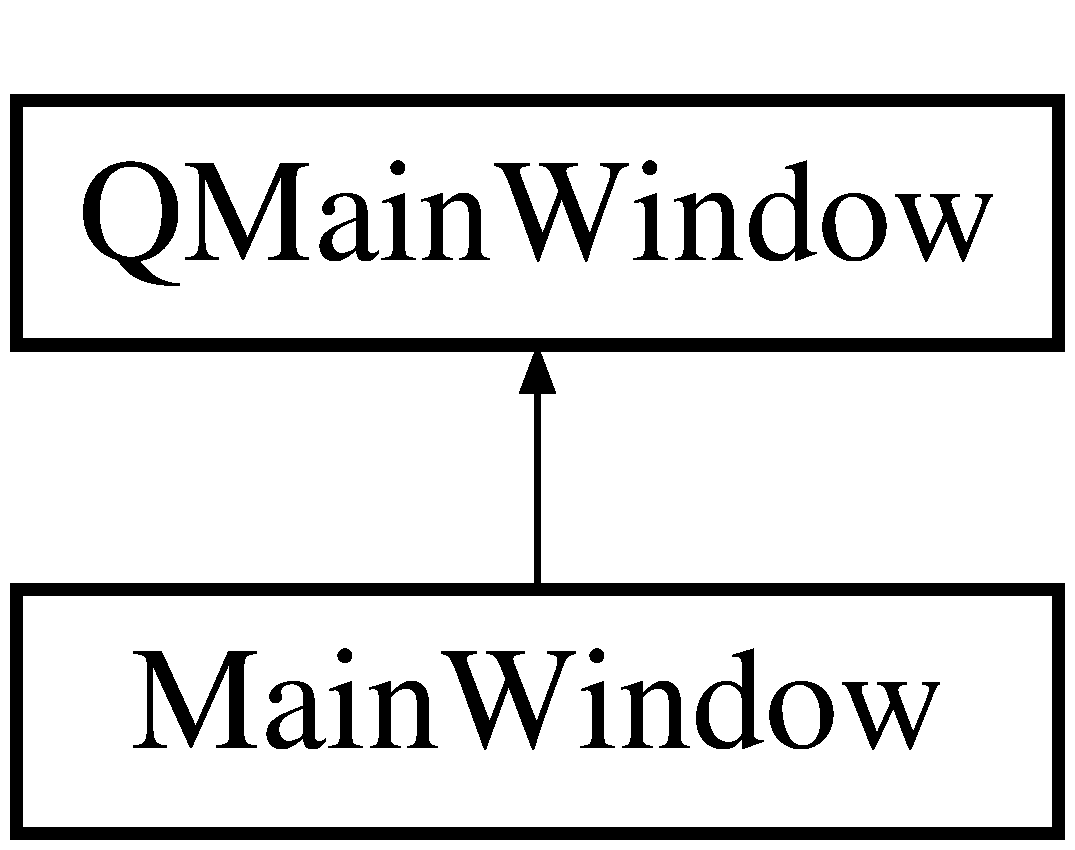
\includegraphics[height=2.000000cm]{class_main_window}
\end{center}
\end{figure}
\subsection*{Public Member Functions}
\begin{DoxyCompactItemize}
\item 
\hypertarget{class_main_window_a8b244be8b7b7db1b08de2a2acb9409db}{{\bfseries Main\+Window} (Q\+Widget $\ast$parent=0)}\label{class_main_window_a8b244be8b7b7db1b08de2a2acb9409db}

\end{DoxyCompactItemize}


\subsection{Detailed Description}
The \hyperlink{class_main_window}{Main\+Window} class Clase encargada del control de la interfaz. 

The documentation for this class was generated from the following files\+:\begin{DoxyCompactItemize}
\item 
mainwindow.\+h\item 
mainwindow.\+cpp\end{DoxyCompactItemize}

\hypertarget{class_matching}{\section{Matching Class Reference}
\label{class_matching}\index{Matching@{Matching}}
}


The \hyperlink{class_matching}{Matching} class Clase que recoge la funcionalidad encargada de realizar el proceso de matchin.  




{\ttfamily \#include $<$matching.\+h$>$}

\subsection*{Public Member Functions}
\begin{DoxyCompactItemize}
\item 
\hypertarget{class_matching_a904a31abfaa75c60e0f5ad5f3d8dec26}{\hyperlink{class_matching_a904a31abfaa75c60e0f5ad5f3d8dec26}{Matching} ()}\label{class_matching_a904a31abfaa75c60e0f5ad5f3d8dec26}

\begin{DoxyCompactList}\small\item\em \hyperlink{class_matching}{Matching} Contructor vacio. \end{DoxyCompactList}\item 
float \hyperlink{class_matching_a2360636756aaf52eea9990cf612d9987}{match} (std\+::vector$<$ \hyperlink{class_minutia}{Minutia} $>$ M1, std\+::vector$<$ \hyperlink{class_minutia}{Minutia} $>$ M2)
\begin{DoxyCompactList}\small\item\em match Metodo que va a realizar el calculo del porcentaje de coincidencia entre dos conjutos de minucias \end{DoxyCompactList}\end{DoxyCompactItemize}


\subsection{Detailed Description}
The \hyperlink{class_matching}{Matching} class Clase que recoge la funcionalidad encargada de realizar el proceso de matchin. 

\subsection{Member Function Documentation}
\hypertarget{class_matching_a2360636756aaf52eea9990cf612d9987}{\index{Matching@{Matching}!match@{match}}
\index{match@{match}!Matching@{Matching}}
\subsubsection[{match}]{\setlength{\rightskip}{0pt plus 5cm}float Matching\+::match (
\begin{DoxyParamCaption}
\item[{std\+::vector$<$ {\bf Minutia} $>$}]{M1, }
\item[{std\+::vector$<$ {\bf Minutia} $>$}]{M2}
\end{DoxyParamCaption}
)}}\label{class_matching_a2360636756aaf52eea9990cf612d9987}


match Metodo que va a realizar el calculo del porcentaje de coincidencia entre dos conjutos de minucias 


\begin{DoxyParams}{Parameters}
{\em M1} & std\+::vector que contiene el primer conjunto de minucias a comparar \\
\hline
{\em M2} & std\+::vector que contiene el segundo conjunto de minucias a comparar \\
\hline
\end{DoxyParams}
\begin{DoxyReturn}{Returns}
Float que indica el porcetanje de coincidencia 
\end{DoxyReturn}


The documentation for this class was generated from the following files\+:\begin{DoxyCompactItemize}
\item 
matching.\+h\item 
matching.\+cpp\end{DoxyCompactItemize}

\hypertarget{class_math_operation}{\section{Math\+Operation Class Reference}
\label{class_math_operation}\index{Math\+Operation@{Math\+Operation}}
}


The \hyperlink{class_math_operation}{Math\+Operation} class Clase en la que se recogen las funciones matematicas necesitadas por el modulo.  




{\ttfamily \#include $<$mathoperation.\+h$>$}

\subsection*{Public Member Functions}
\begin{DoxyCompactItemize}
\item 
\hypertarget{class_math_operation_a06454b3f5ca3dda040cf1e84d57d728c}{\hyperlink{class_math_operation_a06454b3f5ca3dda040cf1e84d57d728c}{Math\+Operation} ()}\label{class_math_operation_a06454b3f5ca3dda040cf1e84d57d728c}

\begin{DoxyCompactList}\small\item\em \hyperlink{class_math_operation}{Math\+Operation} Constructor vacio. \end{DoxyCompactList}\item 
\hyperlink{class_math_operation_a2231defda46af01e401c279d9966de98}{Math\+Operation} (int elements)
\begin{DoxyCompactList}\small\item\em \hyperlink{class_math_operation}{Math\+Operation} Contructor que recibe como argumento el numero de elementos del vector de elementos de la clase. \end{DoxyCompactList}\item 
\hyperlink{class_math_operation_a8d34860d914580697c1100d082e204cc}{Math\+Operation} (int elements, cv\+::\+Mat \&mat)
\begin{DoxyCompactList}\small\item\em \hyperlink{class_math_operation}{Math\+Operation} Contructor que recibe como argumento el numero de elementos del vector de elementos de la clase y la matrix de la image que se va a almacenar en el vector. \end{DoxyCompactList}\item 
double \hyperlink{class_math_operation_afd8a4ec3216a9c1ab0391a1a63002d0d}{Calculate\+Mean} ()
\begin{DoxyCompactList}\small\item\em Calculate\+Mean Metodo que calcula la media del vector de valores de la clase. \end{DoxyCompactList}\item 
double \hyperlink{class_math_operation_a161db6b912577cdcde192eabed812fd8}{Calculate\+Variane} ()
\begin{DoxyCompactList}\small\item\em Calculate\+Variane Metodo que calcula la varianza del vector de valores de la clase. \end{DoxyCompactList}\item 
double \hyperlink{class_math_operation_aab883a9fbdbfe23a539d98089ea27e64}{Get\+Standard\+Deviation} ()
\begin{DoxyCompactList}\small\item\em Get\+Standard\+Deviation Metodo que calcula la desviación tipica del vector de valores de la clase. \end{DoxyCompactList}\item 
double \hyperlink{class_math_operation_a56c06726344749b49944512947036689}{ceil0} (const double \&value)
\begin{DoxyCompactList}\small\item\em ceil0 Metodo que realiza el redondeo al alza y cambiando el signo \end{DoxyCompactList}\item 
double \hyperlink{class_math_operation_a6a719d663bfc475ea89a723a918a8121}{roundhalfup} (const double \&value)
\begin{DoxyCompactList}\small\item\em roundhalfup Metodo que realiza el redondeo al alza sumandole 0.\+5 \end{DoxyCompactList}\item 
double \hyperlink{class_math_operation_aa778c04f56422ba5d0caebc208a7c399}{roundhalfup0} (const double \&value)
\begin{DoxyCompactList}\small\item\em roundhalfup0 Metodo que realiza el redondeo al alza sumandole 0.\+5 y cambiando el signo \end{DoxyCompactList}\item 
double \hyperlink{class_math_operation_a744616f90b70846920b138ef40f0f110}{roundhalfeven} (const double \&value)
\begin{DoxyCompactList}\small\item\em roundhalfeven Metodo que realiza el redondeo del banquero \end{DoxyCompactList}\end{DoxyCompactItemize}
\subsection*{Public Attributes}
\begin{DoxyCompactItemize}
\item 
\hypertarget{class_math_operation_a6c76d3b9b52885d4e7a7712b92224275}{int \hyperlink{class_math_operation_a6c76d3b9b52885d4e7a7712b92224275}{max}}\label{class_math_operation_a6c76d3b9b52885d4e7a7712b92224275}

\begin{DoxyCompactList}\small\item\em max Entero que almacena el numero de elementos \end{DoxyCompactList}\item 
\hypertarget{class_math_operation_af9e269ecc7a79efe7490690dc9e70445}{std\+::vector$<$ double $>$ \hyperlink{class_math_operation_af9e269ecc7a79efe7490690dc9e70445}{values}}\label{class_math_operation_af9e269ecc7a79efe7490690dc9e70445}

\begin{DoxyCompactList}\small\item\em values Vector que almacena los valores de la matriz sobre la que se van a realizar los calculos \end{DoxyCompactList}\item 
\hypertarget{class_math_operation_a1dec04505997677a4dedbf645d4d128c}{double \hyperlink{class_math_operation_a1dec04505997677a4dedbf645d4d128c}{mean}}\label{class_math_operation_a1dec04505997677a4dedbf645d4d128c}

\begin{DoxyCompactList}\small\item\em mean Double que almacena el valor de la media para calculos internos \end{DoxyCompactList}\end{DoxyCompactItemize}


\subsection{Detailed Description}
The \hyperlink{class_math_operation}{Math\+Operation} class Clase en la que se recogen las funciones matematicas necesitadas por el modulo. 

\subsection{Constructor \& Destructor Documentation}
\hypertarget{class_math_operation_a2231defda46af01e401c279d9966de98}{\index{Math\+Operation@{Math\+Operation}!Math\+Operation@{Math\+Operation}}
\index{Math\+Operation@{Math\+Operation}!Math\+Operation@{Math\+Operation}}
\subsubsection[{Math\+Operation}]{\setlength{\rightskip}{0pt plus 5cm}Math\+Operation\+::\+Math\+Operation (
\begin{DoxyParamCaption}
\item[{int}]{elements}
\end{DoxyParamCaption}
)}}\label{class_math_operation_a2231defda46af01e401c279d9966de98}


\hyperlink{class_math_operation}{Math\+Operation} Contructor que recibe como argumento el numero de elementos del vector de elementos de la clase. 


\begin{DoxyParams}{Parameters}
{\em elements} & Numero de elementos que va a tener el vector utilizado para realizar los calculos \\
\hline
\end{DoxyParams}
\hypertarget{class_math_operation_a8d34860d914580697c1100d082e204cc}{\index{Math\+Operation@{Math\+Operation}!Math\+Operation@{Math\+Operation}}
\index{Math\+Operation@{Math\+Operation}!Math\+Operation@{Math\+Operation}}
\subsubsection[{Math\+Operation}]{\setlength{\rightskip}{0pt plus 5cm}Math\+Operation\+::\+Math\+Operation (
\begin{DoxyParamCaption}
\item[{int}]{elements, }
\item[{cv\+::\+Mat \&}]{mat}
\end{DoxyParamCaption}
)}}\label{class_math_operation_a8d34860d914580697c1100d082e204cc}


\hyperlink{class_math_operation}{Math\+Operation} Contructor que recibe como argumento el numero de elementos del vector de elementos de la clase y la matrix de la image que se va a almacenar en el vector. 


\begin{DoxyParams}{Parameters}
{\em elements} & Numero de elementos que va a tener el vector utilizado para realizar los calculos \\
\hline
{\em mat} & cv\+::\+Mat que contiene los valores de la imagen tratados \\
\hline
\end{DoxyParams}


\subsection{Member Function Documentation}
\hypertarget{class_math_operation_afd8a4ec3216a9c1ab0391a1a63002d0d}{\index{Math\+Operation@{Math\+Operation}!Calculate\+Mean@{Calculate\+Mean}}
\index{Calculate\+Mean@{Calculate\+Mean}!Math\+Operation@{Math\+Operation}}
\subsubsection[{Calculate\+Mean}]{\setlength{\rightskip}{0pt plus 5cm}double Math\+Operation\+::\+Calculate\+Mean (
\begin{DoxyParamCaption}
{}
\end{DoxyParamCaption}
)}}\label{class_math_operation_afd8a4ec3216a9c1ab0391a1a63002d0d}


Calculate\+Mean Metodo que calcula la media del vector de valores de la clase. 

\begin{DoxyReturn}{Returns}

\end{DoxyReturn}
\hypertarget{class_math_operation_a161db6b912577cdcde192eabed812fd8}{\index{Math\+Operation@{Math\+Operation}!Calculate\+Variane@{Calculate\+Variane}}
\index{Calculate\+Variane@{Calculate\+Variane}!Math\+Operation@{Math\+Operation}}
\subsubsection[{Calculate\+Variane}]{\setlength{\rightskip}{0pt plus 5cm}double Math\+Operation\+::\+Calculate\+Variane (
\begin{DoxyParamCaption}
{}
\end{DoxyParamCaption}
)}}\label{class_math_operation_a161db6b912577cdcde192eabed812fd8}


Calculate\+Variane Metodo que calcula la varianza del vector de valores de la clase. 

\begin{DoxyReturn}{Returns}

\end{DoxyReturn}
\hypertarget{class_math_operation_a56c06726344749b49944512947036689}{\index{Math\+Operation@{Math\+Operation}!ceil0@{ceil0}}
\index{ceil0@{ceil0}!Math\+Operation@{Math\+Operation}}
\subsubsection[{ceil0}]{\setlength{\rightskip}{0pt plus 5cm}double Math\+Operation\+::ceil0 (
\begin{DoxyParamCaption}
\item[{const double \&}]{value}
\end{DoxyParamCaption}
)}}\label{class_math_operation_a56c06726344749b49944512947036689}


ceil0 Metodo que realiza el redondeo al alza y cambiando el signo 


\begin{DoxyParams}{Parameters}
{\em value} & Valor sobre el que se realiza el calculo \\
\hline
\end{DoxyParams}
\begin{DoxyReturn}{Returns}
Valor calculado 
\end{DoxyReturn}
\hypertarget{class_math_operation_aab883a9fbdbfe23a539d98089ea27e64}{\index{Math\+Operation@{Math\+Operation}!Get\+Standard\+Deviation@{Get\+Standard\+Deviation}}
\index{Get\+Standard\+Deviation@{Get\+Standard\+Deviation}!Math\+Operation@{Math\+Operation}}
\subsubsection[{Get\+Standard\+Deviation}]{\setlength{\rightskip}{0pt plus 5cm}double Math\+Operation\+::\+Get\+Standard\+Deviation (
\begin{DoxyParamCaption}
{}
\end{DoxyParamCaption}
)}}\label{class_math_operation_aab883a9fbdbfe23a539d98089ea27e64}


Get\+Standard\+Deviation Metodo que calcula la desviación tipica del vector de valores de la clase. 

\begin{DoxyReturn}{Returns}

\end{DoxyReturn}
\hypertarget{class_math_operation_a744616f90b70846920b138ef40f0f110}{\index{Math\+Operation@{Math\+Operation}!roundhalfeven@{roundhalfeven}}
\index{roundhalfeven@{roundhalfeven}!Math\+Operation@{Math\+Operation}}
\subsubsection[{roundhalfeven}]{\setlength{\rightskip}{0pt plus 5cm}double Math\+Operation\+::roundhalfeven (
\begin{DoxyParamCaption}
\item[{const double \&}]{value}
\end{DoxyParamCaption}
)}}\label{class_math_operation_a744616f90b70846920b138ef40f0f110}


roundhalfeven Metodo que realiza el redondeo del banquero 


\begin{DoxyParams}{Parameters}
{\em value} & Valor sobre el que se realiza el calculo \\
\hline
\end{DoxyParams}
\begin{DoxyReturn}{Returns}
Valor calculado 
\end{DoxyReturn}
\hypertarget{class_math_operation_a6a719d663bfc475ea89a723a918a8121}{\index{Math\+Operation@{Math\+Operation}!roundhalfup@{roundhalfup}}
\index{roundhalfup@{roundhalfup}!Math\+Operation@{Math\+Operation}}
\subsubsection[{roundhalfup}]{\setlength{\rightskip}{0pt plus 5cm}double Math\+Operation\+::roundhalfup (
\begin{DoxyParamCaption}
\item[{const double \&}]{value}
\end{DoxyParamCaption}
)}}\label{class_math_operation_a6a719d663bfc475ea89a723a918a8121}


roundhalfup Metodo que realiza el redondeo al alza sumandole 0.\+5 


\begin{DoxyParams}{Parameters}
{\em value} & Valor sobre el que se realiza el calculo \\
\hline
\end{DoxyParams}
\begin{DoxyReturn}{Returns}
Valor calculado 
\end{DoxyReturn}
\hypertarget{class_math_operation_aa778c04f56422ba5d0caebc208a7c399}{\index{Math\+Operation@{Math\+Operation}!roundhalfup0@{roundhalfup0}}
\index{roundhalfup0@{roundhalfup0}!Math\+Operation@{Math\+Operation}}
\subsubsection[{roundhalfup0}]{\setlength{\rightskip}{0pt plus 5cm}double Math\+Operation\+::roundhalfup0 (
\begin{DoxyParamCaption}
\item[{const double \&}]{value}
\end{DoxyParamCaption}
)}}\label{class_math_operation_aa778c04f56422ba5d0caebc208a7c399}


roundhalfup0 Metodo que realiza el redondeo al alza sumandole 0.\+5 y cambiando el signo 


\begin{DoxyParams}{Parameters}
{\em value} & Valor sobre el que se realiza el calculo \\
\hline
\end{DoxyParams}
\begin{DoxyReturn}{Returns}
Valor calculado 
\end{DoxyReturn}


The documentation for this class was generated from the following files\+:\begin{DoxyCompactItemize}
\item 
mathoperation.\+h\item 
mathoperation.\+cpp\end{DoxyCompactItemize}

\hypertarget{class_minutia}{\section{Minutia Class Reference}
\label{class_minutia}\index{Minutia@{Minutia}}
}


The \hyperlink{class_minutia}{Minutia} class Clase que va a contener las caracteristicas de la minucias.  




{\ttfamily \#include $<$minutia.\+h$>$}

\subsection*{Public Member Functions}
\begin{DoxyCompactItemize}
\item 
\hypertarget{class_minutia_a0b52999eded30030b53e912bfdb38dc6}{\hyperlink{class_minutia_a0b52999eded30030b53e912bfdb38dc6}{Minutia} ()}\label{class_minutia_a0b52999eded30030b53e912bfdb38dc6}

\begin{DoxyCompactList}\small\item\em \hyperlink{class_minutia}{Minutia} Constructor vacio. \end{DoxyCompactList}\item 
\hyperlink{class_minutia_aae46fc644b6024bd26847f49dd40aef0}{Minutia} (double an, int x\+\_\+pos, int y\+\_\+pos, Minutia\+Type t)
\begin{DoxyCompactList}\small\item\em \hyperlink{class_minutia}{Minutia} Contructor con argumentos para crear los objetos tipo minucia. \end{DoxyCompactList}\item 
\hyperlink{class_minutia_ab63ae144e73b87457e0660ab85591a8f}{Minutia} (double an, int x\+\_\+pos, int y\+\_\+pos)
\begin{DoxyCompactList}\small\item\em \hyperlink{class_minutia}{Minutia} Contructor con argumentos para crear los objetos tipo minucia. \end{DoxyCompactList}\end{DoxyCompactItemize}
\subsection*{Public Attributes}
\begin{DoxyCompactItemize}
\item 
\hypertarget{class_minutia_a50aa5fe07287adcc5106755e68f437dd}{float \hyperlink{class_minutia_a50aa5fe07287adcc5106755e68f437dd}{angle}}\label{class_minutia_a50aa5fe07287adcc5106755e68f437dd}

\begin{DoxyCompactList}\small\item\em angle Double que almacena la orientacion de la minucia \end{DoxyCompactList}\item 
\hypertarget{class_minutia_a64e1e7a198334f923b9ae536cf6348bd}{float \hyperlink{class_minutia_a64e1e7a198334f923b9ae536cf6348bd}{x}}\label{class_minutia_a64e1e7a198334f923b9ae536cf6348bd}

\begin{DoxyCompactList}\small\item\em x Entero que almacena la posicion de la minucia en el eje x \end{DoxyCompactList}\item 
\hypertarget{class_minutia_acce51490952cc57448b6fa861d4632bd}{float \hyperlink{class_minutia_acce51490952cc57448b6fa861d4632bd}{y}}\label{class_minutia_acce51490952cc57448b6fa861d4632bd}

\begin{DoxyCompactList}\small\item\em y Entero que almacena la posicion de la minucia en el eje y \end{DoxyCompactList}\item 
\hypertarget{class_minutia_a7f467139e7cd3928ebc71c3e2d4e3d7f}{Minutia\+Type \hyperlink{class_minutia_a7f467139e7cd3928ebc71c3e2d4e3d7f}{type}}\label{class_minutia_a7f467139e7cd3928ebc71c3e2d4e3d7f}

\begin{DoxyCompactList}\small\item\em type Valor que indica el tipo de minucia \end{DoxyCompactList}\end{DoxyCompactItemize}


\subsection{Detailed Description}
The \hyperlink{class_minutia}{Minutia} class Clase que va a contener las caracteristicas de la minucias. 

\subsection{Constructor \& Destructor Documentation}
\hypertarget{class_minutia_aae46fc644b6024bd26847f49dd40aef0}{\index{Minutia@{Minutia}!Minutia@{Minutia}}
\index{Minutia@{Minutia}!Minutia@{Minutia}}
\subsubsection[{Minutia}]{\setlength{\rightskip}{0pt plus 5cm}Minutia\+::\+Minutia (
\begin{DoxyParamCaption}
\item[{double}]{an, }
\item[{int}]{x\+\_\+pos, }
\item[{int}]{y\+\_\+pos, }
\item[{Minutia\+Type}]{t}
\end{DoxyParamCaption}
)}}\label{class_minutia_aae46fc644b6024bd26847f49dd40aef0}


\hyperlink{class_minutia}{Minutia} Contructor con argumentos para crear los objetos tipo minucia. 


\begin{DoxyParams}{Parameters}
{\em an} & Double que indica el angulo de la minucia \\
\hline
{\em x\+\_\+pos} & Entero que indica la posicion de la minucia en el eje x \\
\hline
{\em y\+\_\+pos} & Entero que indica la posicion de la minucia en el eje y \\
\hline
{\em t} & Tipo de minucia \\
\hline
\end{DoxyParams}
\hypertarget{class_minutia_ab63ae144e73b87457e0660ab85591a8f}{\index{Minutia@{Minutia}!Minutia@{Minutia}}
\index{Minutia@{Minutia}!Minutia@{Minutia}}
\subsubsection[{Minutia}]{\setlength{\rightskip}{0pt plus 5cm}Minutia\+::\+Minutia (
\begin{DoxyParamCaption}
\item[{double}]{an, }
\item[{int}]{x\+\_\+pos, }
\item[{int}]{y\+\_\+pos}
\end{DoxyParamCaption}
)}}\label{class_minutia_ab63ae144e73b87457e0660ab85591a8f}


\hyperlink{class_minutia}{Minutia} Contructor con argumentos para crear los objetos tipo minucia. 


\begin{DoxyParams}{Parameters}
{\em an} & Double que indica el angulo de la minucia \\
\hline
{\em x\+\_\+pos} & Entero que indica la posicion de la minucia en el eje x \\
\hline
{\em y\+\_\+pos} & Entero que indica la posicion de la minucia en el eje y \\
\hline
\end{DoxyParams}


The documentation for this class was generated from the following files\+:\begin{DoxyCompactItemize}
\item 
minutia.\+h\item 
minutia.\+cpp\end{DoxyCompactItemize}

\hypertarget{class_minutia_extractor}{\section{Minutia\+Extractor Class Reference}
\label{class_minutia_extractor}\index{Minutia\+Extractor@{Minutia\+Extractor}}
}


The \hyperlink{class_minutia_extractor}{Minutia\+Extractor} class Clase que recoge la funcionalidad encargada de realizar la extraccion de minucias de la imagen.  




{\ttfamily \#include $<$minutiaextractor.\+h$>$}

\subsection*{Public Member Functions}
\begin{DoxyCompactItemize}
\item 
\hypertarget{class_minutia_extractor_adccd8fca1f1718e7b736f158700d432a}{\hyperlink{class_minutia_extractor_adccd8fca1f1718e7b736f158700d432a}{Minutia\+Extractor} ()}\label{class_minutia_extractor_adccd8fca1f1718e7b736f158700d432a}

\begin{DoxyCompactList}\small\item\em \hyperlink{class_minutia_extractor}{Minutia\+Extractor} Constructor vacio. \end{DoxyCompactList}\item 
std\+::vector$<$ \hyperlink{class_minutia}{Minutia} $>$ \hyperlink{class_minutia_extractor_adbde01c42359f1cddc3d8cb99f09f5d9}{extract\+Minutiae} (cv\+::\+Mat \&matrix, cv\+::\+Mat \&orientation\+Image, cv\+::\+Mat \&segment, int block\+Size)
\begin{DoxyCompactList}\small\item\em extract\+Minutia Metodo que realiza la extraccion de minucias sobre una huella dactilar \end{DoxyCompactList}\item 
void \hyperlink{class_minutia_extractor_aa71d473dd4dcf6559a47765d17e16d5f}{overlay\+Minutiae} (std\+::vector$<$ \hyperlink{class_minutia}{Minutia} $>$ features, cv\+::\+Mat \&img)
\begin{DoxyCompactList}\small\item\em Show Metodo que muestra las minucias sobre la imagen de la huella dactilar. \end{DoxyCompactList}\item 
void \hyperlink{class_minutia_extractor_a7010ac95bbbfa607897eef04acc5e9aa}{compare\+Fingerprint\+Minutiae} (std\+::vector$<$ \hyperlink{class_minutia}{Minutia} $>$ features, cv\+::\+Mat \&img, int number\+Image)
\begin{DoxyCompactList}\small\item\em compare\+Fingerprint\+Minutiaes Metodo que muestra la compracion entre dos conjuntos de minucias \end{DoxyCompactList}\end{DoxyCompactItemize}
\subsection*{Public Attributes}
\begin{DoxyCompactItemize}
\item 
\hypertarget{class_minutia_extractor_a6f8e432d15f8b6758a38438d59462cfc}{std\+::vector$<$ \hyperlink{class_minutia}{Minutia} $>$ \hyperlink{class_minutia_extractor_a6f8e432d15f8b6758a38438d59462cfc}{minutiae}}\label{class_minutia_extractor_a6f8e432d15f8b6758a38438d59462cfc}

\begin{DoxyCompactList}\small\item\em minutiae Vector en el que se van a almacenar minucias \end{DoxyCompactList}\end{DoxyCompactItemize}


\subsection{Detailed Description}
The \hyperlink{class_minutia_extractor}{Minutia\+Extractor} class Clase que recoge la funcionalidad encargada de realizar la extraccion de minucias de la imagen. 

\subsection{Member Function Documentation}
\hypertarget{class_minutia_extractor_a7010ac95bbbfa607897eef04acc5e9aa}{\index{Minutia\+Extractor@{Minutia\+Extractor}!compare\+Fingerprint\+Minutiae@{compare\+Fingerprint\+Minutiae}}
\index{compare\+Fingerprint\+Minutiae@{compare\+Fingerprint\+Minutiae}!Minutia\+Extractor@{Minutia\+Extractor}}
\subsubsection[{compare\+Fingerprint\+Minutiae}]{\setlength{\rightskip}{0pt plus 5cm}void Minutia\+Extractor\+::compare\+Fingerprint\+Minutiae (
\begin{DoxyParamCaption}
\item[{std\+::vector$<$ {\bf Minutia} $>$}]{features, }
\item[{cv\+::\+Mat \&}]{img, }
\item[{int}]{number\+Image}
\end{DoxyParamCaption}
)}}\label{class_minutia_extractor_a7010ac95bbbfa607897eef04acc5e9aa}


compare\+Fingerprint\+Minutiaes Metodo que muestra la compracion entre dos conjuntos de minucias 


\begin{DoxyParams}{Parameters}
{\em features} & Vector de minucias \\
\hline
{\em img} & cv\+::\+Mat sobre la que se muestran las minucias \\
\hline
{\em number\+Image} & Imagen que se va a tratar \\
\hline
\end{DoxyParams}
\hypertarget{class_minutia_extractor_adbde01c42359f1cddc3d8cb99f09f5d9}{\index{Minutia\+Extractor@{Minutia\+Extractor}!extract\+Minutiae@{extract\+Minutiae}}
\index{extract\+Minutiae@{extract\+Minutiae}!Minutia\+Extractor@{Minutia\+Extractor}}
\subsubsection[{extract\+Minutiae}]{\setlength{\rightskip}{0pt plus 5cm}std\+::vector$<$ {\bf Minutia} $>$ Minutia\+Extractor\+::extract\+Minutiae (
\begin{DoxyParamCaption}
\item[{cv\+::\+Mat \&}]{matrix, }
\item[{cv\+::\+Mat \&}]{orientation\+Image, }
\item[{cv\+::\+Mat \&}]{segment, }
\item[{int}]{block\+Size}
\end{DoxyParamCaption}
)}}\label{class_minutia_extractor_adbde01c42359f1cddc3d8cb99f09f5d9}


extract\+Minutia Metodo que realiza la extraccion de minucias sobre una huella dactilar 

\begin{DoxyReturn}{Returns}
Vector con las minucias extraidads 
\end{DoxyReturn}
Se recorren los bloques de imagen si la orientación es no nula

Se recorren los pixels de cada bloque

Si el pixel es de color negro se calcula su C\+N

Minucia de tipo final, se comprueba si es verdadera y se añade

Minucia de tipo bifurcacion, se comprueba si es verdadera y se añade

Se eliminan las minucias que coinciden en los bordes de las crestas

Se eliminan las falsas minucias minucias\hypertarget{class_minutia_extractor_aa71d473dd4dcf6559a47765d17e16d5f}{\index{Minutia\+Extractor@{Minutia\+Extractor}!overlay\+Minutiae@{overlay\+Minutiae}}
\index{overlay\+Minutiae@{overlay\+Minutiae}!Minutia\+Extractor@{Minutia\+Extractor}}
\subsubsection[{overlay\+Minutiae}]{\setlength{\rightskip}{0pt plus 5cm}void Minutia\+Extractor\+::overlay\+Minutiae (
\begin{DoxyParamCaption}
\item[{std\+::vector$<$ {\bf Minutia} $>$}]{features, }
\item[{cv\+::\+Mat \&}]{img}
\end{DoxyParamCaption}
)}}\label{class_minutia_extractor_aa71d473dd4dcf6559a47765d17e16d5f}


Show Metodo que muestra las minucias sobre la imagen de la huella dactilar. 


\begin{DoxyParams}{Parameters}
{\em features} & Vector de minucias \\
\hline
{\em img} & cv\+::\+Mat sobre la que se muestran las minucias \\
\hline
\end{DoxyParams}


The documentation for this class was generated from the following files\+:\begin{DoxyCompactItemize}
\item 
minutiaextractor.\+h\item 
minutiaextractor.\+cpp\end{DoxyCompactItemize}

\hypertarget{class_normalize}{\section{Normalize Class Reference}
\label{class_normalize}\index{Normalize@{Normalize}}
}


The \hyperlink{class_normalize}{Normalize} class Clase que recoge la funcionalidad encargada de realizar la normalizacion de la imagen.  




{\ttfamily \#include $<$normalize.\+h$>$}

\subsection*{Public Member Functions}
\begin{DoxyCompactItemize}
\item 
\hypertarget{class_normalize_a4e02803bd3999792686b756d8a486a6a}{\hyperlink{class_normalize_a4e02803bd3999792686b756d8a486a6a}{Normalize} ()}\label{class_normalize_a4e02803bd3999792686b756d8a486a6a}

\begin{DoxyCompactList}\small\item\em \hyperlink{class_normalize}{Normalize} Contructor vacio. \end{DoxyCompactList}\item 
void \hyperlink{class_normalize_a280fff45c1f616b80f1f5fce8006906c}{normalizacion} (cv\+::\+Mat \&src)
\begin{DoxyCompactList}\small\item\em normalizacion Metodo que realiza el calculo de la normalizacion de la imagen recibida como parametro \end{DoxyCompactList}\item 
void \hyperlink{class_normalize_a03e2994ccaf935c43bc3eebcc3ba0369}{normalizacion\+Mask} (cv\+::\+Mat \&src)
\begin{DoxyCompactList}\small\item\em normalizacion\+Mask Metodo que calcula la mascara de normalizacion a partir de la varianza \end{DoxyCompactList}\end{DoxyCompactItemize}


\subsection{Detailed Description}
The \hyperlink{class_normalize}{Normalize} class Clase que recoge la funcionalidad encargada de realizar la normalizacion de la imagen. 

\subsection{Member Function Documentation}
\hypertarget{class_normalize_a280fff45c1f616b80f1f5fce8006906c}{\index{Normalize@{Normalize}!normalizacion@{normalizacion}}
\index{normalizacion@{normalizacion}!Normalize@{Normalize}}
\subsubsection[{normalizacion}]{\setlength{\rightskip}{0pt plus 5cm}void Normalize\+::normalizacion (
\begin{DoxyParamCaption}
\item[{cv\+::\+Mat \&}]{src}
\end{DoxyParamCaption}
)}}\label{class_normalize_a280fff45c1f616b80f1f5fce8006906c}


normalizacion Metodo que realiza el calculo de la normalizacion de la imagen recibida como parametro 


\begin{DoxyParams}{Parameters}
{\em src} & cv\+::\+Mat de entrada \\
\hline
\end{DoxyParams}
\hypertarget{class_normalize_a03e2994ccaf935c43bc3eebcc3ba0369}{\index{Normalize@{Normalize}!normalizacion\+Mask@{normalizacion\+Mask}}
\index{normalizacion\+Mask@{normalizacion\+Mask}!Normalize@{Normalize}}
\subsubsection[{normalizacion\+Mask}]{\setlength{\rightskip}{0pt plus 5cm}void Normalize\+::normalizacion\+Mask (
\begin{DoxyParamCaption}
\item[{cv\+::\+Mat \&}]{src}
\end{DoxyParamCaption}
)}}\label{class_normalize_a03e2994ccaf935c43bc3eebcc3ba0369}


normalizacion\+Mask Metodo que calcula la mascara de normalizacion a partir de la varianza 


\begin{DoxyParams}{Parameters}
{\em src} & cv\+::\+Mat de entrada \\
\hline
\end{DoxyParams}


The documentation for this class was generated from the following files\+:\begin{DoxyCompactItemize}
\item 
normalize.\+h\item 
normalize.\+cpp\end{DoxyCompactItemize}

\hypertarget{class_orientation}{\section{Orientation Class Reference}
\label{class_orientation}\index{Orientation@{Orientation}}
}


The \hyperlink{class_orientation}{Orientation} class Clase que recoge la funcionalidad encargada de realizar la orientacion de la imagen.  




{\ttfamily \#include $<$orientation.\+h$>$}

\subsection*{Public Member Functions}
\begin{DoxyCompactItemize}
\item 
\hypertarget{class_orientation_afa8e101af342cdf57d5e33109ffc6529}{\hyperlink{class_orientation_afa8e101af342cdf57d5e33109ffc6529}{Orientation} ()}\label{class_orientation_afa8e101af342cdf57d5e33109ffc6529}

\begin{DoxyCompactList}\small\item\em \hyperlink{class_orientation}{Orientation} Constructor vacio. \end{DoxyCompactList}\item 
void \hyperlink{class_orientation_a16a1fdfd5c484d5b1ecb574f033beca1}{calculate\+Orientation} (cv\+::\+Mat \&src, int block\+Size)
\begin{DoxyCompactList}\small\item\em calculate\+Orientation Metodo encargado de calculo de la orientacion por bloques \end{DoxyCompactList}\item 
void \hyperlink{class_orientation_ae7596eaf11b2e9c622a5df1ac9433257}{overlay\+Orientation} (cv\+::\+Mat \&src, cv\+::\+Mat \&oi, int block\+Size)
\begin{DoxyCompactList}\small\item\em overlay\+Orientation Metodo que dibuja la orientacion sobre la matriz original \end{DoxyCompactList}\item 
void \hyperlink{class_orientation_a0496e614c6a189d19ce9cc4577e6fc08}{overlay\+Orientation\+Pixel} (cv\+::\+Mat \&src, cv\+::\+Mat \&oi, int block\+Size)
\begin{DoxyCompactList}\small\item\em overlay\+Orientation\+Pixel Metodo que dibuja la orientacion sobre la matriz original \end{DoxyCompactList}\item 
void \hyperlink{class_orientation_af60f0c95c27fadd864c533c9effd648b}{overlay\+Orientation\+Block} (cv\+::\+Mat \&src, cv\+::\+Mat \&oi, int block\+Size)
\begin{DoxyCompactList}\small\item\em overlay\+Orientation\+Block Metodo que dibuja la orientacion sobre la matriz original \end{DoxyCompactList}\item 
void \hyperlink{class_orientation_afbed70e624322d718d685390d9631b31}{calculate\+Orientation\+Pixel} (cv\+::\+Mat \&src, int block\+Size)
\begin{DoxyCompactList}\small\item\em calculate\+Orientation\+Pixel Metodo encargado de calculo de la orientacion por pixeles \end{DoxyCompactList}\item 
void \hyperlink{class_orientation_aeefb88e6e17f4ee98d469dcd3375ab6c}{calculate\+Orientation\+Block} (cv\+::\+Mat \&src, int block\+Size)
\begin{DoxyCompactList}\small\item\em calculate\+Orientation\+Block Metodo encargado de calculo de la orientacion por bloques menos eficiente \end{DoxyCompactList}\end{DoxyCompactItemize}
\subsection*{Public Attributes}
\begin{DoxyCompactItemize}
\item 
\hypertarget{class_orientation_a3bf906cb5bae4d9cfcb99512bb348086}{cv\+::\+Mat \hyperlink{class_orientation_a3bf906cb5bae4d9cfcb99512bb348086}{oi\+Matrix}}\label{class_orientation_a3bf906cb5bae4d9cfcb99512bb348086}

\begin{DoxyCompactList}\small\item\em oi\+Matrix cv\+::\+Mat que almacena la orientacion calculada \end{DoxyCompactList}\item 
\hypertarget{class_orientation_a2ea4cd6254ecfb1123db119cdfad38a3}{cv\+::\+Mat \hyperlink{class_orientation_a2ea4cd6254ecfb1123db119cdfad38a3}{oi\+Matrix\+Pixel}}\label{class_orientation_a2ea4cd6254ecfb1123db119cdfad38a3}

\begin{DoxyCompactList}\small\item\em oi\+Matrix\+Pixel cv\+::\+Mat que almacena la orientacion calculada mediante el metodo de pixel \end{DoxyCompactList}\item 
\hypertarget{class_orientation_af2d86f34c6597d55149fb729ef02c587}{cv\+::\+Mat \hyperlink{class_orientation_af2d86f34c6597d55149fb729ef02c587}{oi\+Matrix\+Block}}\label{class_orientation_af2d86f34c6597d55149fb729ef02c587}

\begin{DoxyCompactList}\small\item\em oi\+Matrix\+Block cv\+::\+Mat que almacena la orientacion calculada mediante el metodo de bloque menos eficiente \end{DoxyCompactList}\end{DoxyCompactItemize}


\subsection{Detailed Description}
The \hyperlink{class_orientation}{Orientation} class Clase que recoge la funcionalidad encargada de realizar la orientacion de la imagen. 

\subsection{Member Function Documentation}
\hypertarget{class_orientation_a16a1fdfd5c484d5b1ecb574f033beca1}{\index{Orientation@{Orientation}!calculate\+Orientation@{calculate\+Orientation}}
\index{calculate\+Orientation@{calculate\+Orientation}!Orientation@{Orientation}}
\subsubsection[{calculate\+Orientation}]{\setlength{\rightskip}{0pt plus 5cm}void Orientation\+::calculate\+Orientation (
\begin{DoxyParamCaption}
\item[{cv\+::\+Mat \&}]{src, }
\item[{int}]{block\+Size}
\end{DoxyParamCaption}
)}}\label{class_orientation_a16a1fdfd5c484d5b1ecb574f033beca1}


calculate\+Orientation Metodo encargado de calculo de la orientacion por bloques 


\begin{DoxyParams}{Parameters}
{\em src} & cv\+::\+Mat que contiene la imagen sobre la que se va a calcular la orientacion \\
\hline
\end{DoxyParams}
Filtro pasa baja

Gradient X

Gradient Y

Calculate orientations of gradients --$>$ in degrees Loop over all matrix values and calculate the accompanied orientation

Ponemos $<$= si para que recorra hasta el final Podriamos haber empezado en block/2-\/1 y acabar en $<$ \hypertarget{class_orientation_aeefb88e6e17f4ee98d469dcd3375ab6c}{\index{Orientation@{Orientation}!calculate\+Orientation\+Block@{calculate\+Orientation\+Block}}
\index{calculate\+Orientation\+Block@{calculate\+Orientation\+Block}!Orientation@{Orientation}}
\subsubsection[{calculate\+Orientation\+Block}]{\setlength{\rightskip}{0pt plus 5cm}void Orientation\+::calculate\+Orientation\+Block (
\begin{DoxyParamCaption}
\item[{cv\+::\+Mat \&}]{src, }
\item[{int}]{block\+Size}
\end{DoxyParamCaption}
)}}\label{class_orientation_aeefb88e6e17f4ee98d469dcd3375ab6c}


calculate\+Orientation\+Block Metodo encargado de calculo de la orientacion por bloques menos eficiente 


\begin{DoxyParams}{Parameters}
{\em src} & cv\+::\+Mat que contiene la imagen sobre la que se va a calcular la orientacion \\
\hline
{\em block\+Size} & Entero que almacena el tamaño del bloque de la orientacion \\
\hline
\end{DoxyParams}
\hypertarget{class_orientation_afbed70e624322d718d685390d9631b31}{\index{Orientation@{Orientation}!calculate\+Orientation\+Pixel@{calculate\+Orientation\+Pixel}}
\index{calculate\+Orientation\+Pixel@{calculate\+Orientation\+Pixel}!Orientation@{Orientation}}
\subsubsection[{calculate\+Orientation\+Pixel}]{\setlength{\rightskip}{0pt plus 5cm}void Orientation\+::calculate\+Orientation\+Pixel (
\begin{DoxyParamCaption}
\item[{cv\+::\+Mat \&}]{src, }
\item[{int}]{block\+Size}
\end{DoxyParamCaption}
)}}\label{class_orientation_afbed70e624322d718d685390d9631b31}


calculate\+Orientation\+Pixel Metodo encargado de calculo de la orientacion por pixeles 


\begin{DoxyParams}{Parameters}
{\em src} & cv\+::\+Mat que contiene la imagen sobre la que se va a calcular la orientacion \\
\hline
{\em block\+Size} & Entero que almacena el tamaño del bloque de la orientacion \\
\hline
\end{DoxyParams}
\hypertarget{class_orientation_ae7596eaf11b2e9c622a5df1ac9433257}{\index{Orientation@{Orientation}!overlay\+Orientation@{overlay\+Orientation}}
\index{overlay\+Orientation@{overlay\+Orientation}!Orientation@{Orientation}}
\subsubsection[{overlay\+Orientation}]{\setlength{\rightskip}{0pt plus 5cm}void Orientation\+::overlay\+Orientation (
\begin{DoxyParamCaption}
\item[{cv\+::\+Mat \&}]{src, }
\item[{cv\+::\+Mat \&}]{oi, }
\item[{int}]{block\+Size}
\end{DoxyParamCaption}
)}}\label{class_orientation_ae7596eaf11b2e9c622a5df1ac9433257}


overlay\+Orientation Metodo que dibuja la orientacion sobre la matriz original 


\begin{DoxyParams}{Parameters}
{\em src} & cv\+::\+Mat que contiene la imagen original \\
\hline
{\em oi} & cv\+::\+Mat que contine la orientacion de la imagen \\
\hline
{\em block\+Size} & Entero que almacena el tamaño del bloque de la orientacion \\
\hline
\end{DoxyParams}
\hypertarget{class_orientation_af60f0c95c27fadd864c533c9effd648b}{\index{Orientation@{Orientation}!overlay\+Orientation\+Block@{overlay\+Orientation\+Block}}
\index{overlay\+Orientation\+Block@{overlay\+Orientation\+Block}!Orientation@{Orientation}}
\subsubsection[{overlay\+Orientation\+Block}]{\setlength{\rightskip}{0pt plus 5cm}void Orientation\+::overlay\+Orientation\+Block (
\begin{DoxyParamCaption}
\item[{cv\+::\+Mat \&}]{src, }
\item[{cv\+::\+Mat \&}]{oi, }
\item[{int}]{block\+Size}
\end{DoxyParamCaption}
)}}\label{class_orientation_af60f0c95c27fadd864c533c9effd648b}


overlay\+Orientation\+Block Metodo que dibuja la orientacion sobre la matriz original 


\begin{DoxyParams}{Parameters}
{\em src} & cv\+::\+Mat que contiene la imagen original \\
\hline
{\em oi} & cv\+::\+Mat que contine la orientacion de la imagen \\
\hline
{\em block\+Size} & Entero que almacena el tamaño del bloque de la orientacion \\
\hline
\end{DoxyParams}
\hypertarget{class_orientation_a0496e614c6a189d19ce9cc4577e6fc08}{\index{Orientation@{Orientation}!overlay\+Orientation\+Pixel@{overlay\+Orientation\+Pixel}}
\index{overlay\+Orientation\+Pixel@{overlay\+Orientation\+Pixel}!Orientation@{Orientation}}
\subsubsection[{overlay\+Orientation\+Pixel}]{\setlength{\rightskip}{0pt plus 5cm}void Orientation\+::overlay\+Orientation\+Pixel (
\begin{DoxyParamCaption}
\item[{cv\+::\+Mat \&}]{src, }
\item[{cv\+::\+Mat \&}]{oi, }
\item[{int}]{block\+Size}
\end{DoxyParamCaption}
)}}\label{class_orientation_a0496e614c6a189d19ce9cc4577e6fc08}


overlay\+Orientation\+Pixel Metodo que dibuja la orientacion sobre la matriz original 


\begin{DoxyParams}{Parameters}
{\em src} & cv\+::\+Mat que contiene la imagen original \\
\hline
{\em oi} & cv\+::\+Mat que contine la orientacion de la imagen \\
\hline
{\em block\+Size} & Entero que almacena el tamaño del bloque de la orientacion \\
\hline
\end{DoxyParams}


The documentation for this class was generated from the following files\+:\begin{DoxyCompactItemize}
\item 
orientation.\+h\item 
orientation.\+cpp\end{DoxyCompactItemize}

\hypertarget{class_process_fingerprint}{\section{Process\+Fingerprint Class Reference}
\label{class_process_fingerprint}\index{Process\+Fingerprint@{Process\+Fingerprint}}
}


The \hyperlink{class_process_fingerprint}{Process\+Fingerprint} class Clase que recoge la funcionalidad encargada de encamsular el procesamiento de la imagen.  




{\ttfamily \#include $<$processfingerprint.\+h$>$}

Inheritance diagram for Process\+Fingerprint\+:\begin{figure}[H]
\begin{center}
\leavevmode
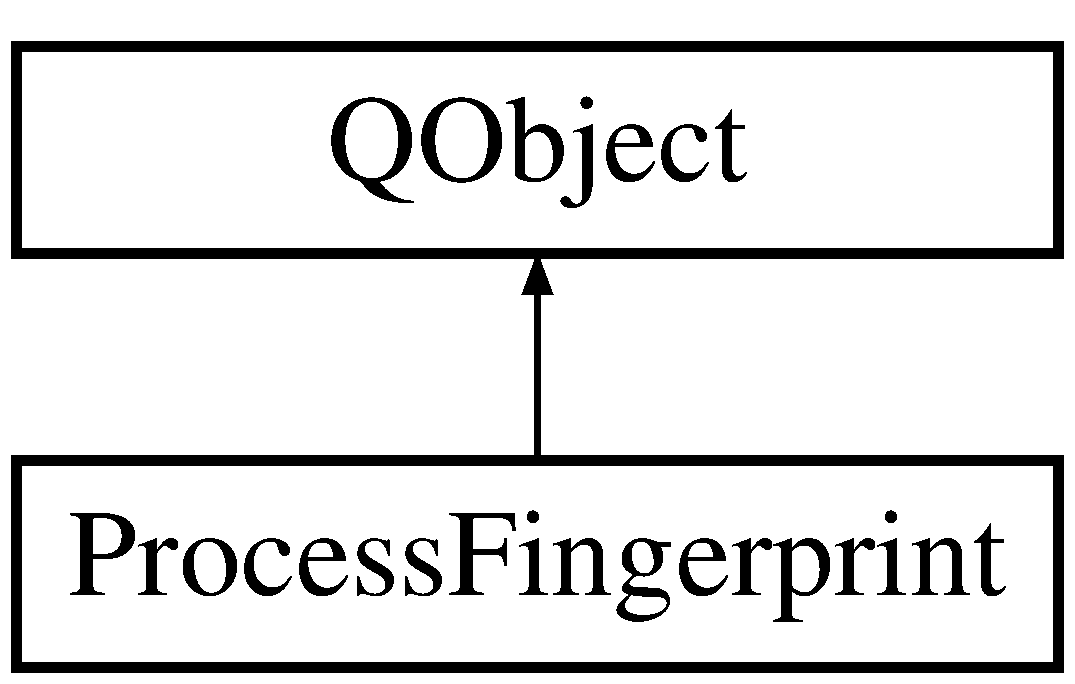
\includegraphics[height=2.000000cm]{class_process_fingerprint}
\end{center}
\end{figure}
\subsection*{Signals}
\begin{DoxyCompactItemize}
\item 
\hypertarget{class_process_fingerprint_a0aab549a54402a9af407f74f5ab88ed5}{void \hyperlink{class_process_fingerprint_a0aab549a54402a9af407f74f5ab88ed5}{finished\+Process\+Fingerprint} (void)}\label{class_process_fingerprint_a0aab549a54402a9af407f74f5ab88ed5}

\begin{DoxyCompactList}\small\item\em finished\+Process\+Fingerprint Señal emitida cuando termina el procesamiento \end{DoxyCompactList}\item 
void \hyperlink{class_process_fingerprint_af40be3dc9ad1557aec8d143280ffbe37}{progress\+Value\+Process\+Fingerprint} (Q\+String message)
\begin{DoxyCompactList}\small\item\em progress\+Value\+Process\+Fingerprint Señal emitida duarnte el procesamiento \end{DoxyCompactList}\item 
\hypertarget{class_process_fingerprint_aae2a751a3dd9ac41755df94212483f4d}{void \hyperlink{class_process_fingerprint_aae2a751a3dd9ac41755df94212483f4d}{finished\+Fingerprint\+Comparison} (void)}\label{class_process_fingerprint_aae2a751a3dd9ac41755df94212483f4d}

\begin{DoxyCompactList}\small\item\em finished\+Fingerprint\+Comparison Señal emitida cuando termina el proceso de compracion \end{DoxyCompactList}\item 
void \hyperlink{class_process_fingerprint_a888be8ba7023f86c4dab1c6b037d5066}{progress\+Value\+Compare\+Fingerprints} (Q\+String message)
\begin{DoxyCompactList}\small\item\em progress\+Value\+Compare\+Fingerprints Señal emitida duarnte el proceso de comparacion \end{DoxyCompactList}\end{DoxyCompactItemize}
\subsection*{Public Member Functions}
\begin{DoxyCompactItemize}
\item 
\hyperlink{class_process_fingerprint_ae2a1238e3736f8959eee3be36727f1f4}{Process\+Fingerprint} (Q\+Object $\ast$parent=0)
\begin{DoxyCompactList}\small\item\em \hyperlink{class_process_fingerprint}{Process\+Fingerprint} Contructor. \end{DoxyCompactList}\item 
void \hyperlink{class_process_fingerprint_a64482c12a72baede08336ce94a63ca06}{process} (Q\+String\+List images\+Names, int tam)
\begin{DoxyCompactList}\small\item\em process Metodo que realiza el procesamiento de la imagen original calculando todas la imagenes intermedias \end{DoxyCompactList}\item 
void \hyperlink{class_process_fingerprint_a64c17de334d4cb1c8193eb970abecffe}{obtain\+Minutiae\+From\+Source\+Image} (cv\+::\+Mat \&color, int tam, std\+::vector$<$ \hyperlink{class_minutia}{Minutia} $>$ \&minutiaes, int number\+Image, Image\+Source source)
\begin{DoxyCompactList}\small\item\em obtain\+Minutiae\+From\+Source\+Image Metodo que calcula las minucias de la imagen original \end{DoxyCompactList}\item 
void \hyperlink{class_process_fingerprint_a5e64ed1959421c4240c9281127d1d2fb}{obtain\+Minutiae\+From\+Source\+Image\+Async} (cv\+::\+Mat \&color, int tam)
\begin{DoxyCompactList}\small\item\em obtain\+Minutiae\+From\+Source\+Image\+Async \end{DoxyCompactList}\item 
cv\+::\+Mat \hyperlink{class_process_fingerprint_aa860148cdae1ab342c8e6c272a4bed64}{resize} (cv\+::\+Mat \&src, int tam)
\begin{DoxyCompactList}\small\item\em resize Metodo que recalcula el tamaño de la imagen \end{DoxyCompactList}\item 
cv\+::\+Mat \hyperlink{class_process_fingerprint_a7fc64b7aa73ddca798de4bf0ffed3794}{to\+Black\+And\+White} (cv\+::\+Mat \&src)
\begin{DoxyCompactList}\small\item\em to\+Black\+And\+White Metodo que transforma la imagen a escala de grises \end{DoxyCompactList}\item 
void \hyperlink{class_process_fingerprint_a50eaef1419b0158557d2c69cc0de9158}{match} (cv\+::\+Mat \&left\+Image, cv\+::\+Mat \&right\+Image)
\begin{DoxyCompactList}\small\item\em match Metodo calcla el porcentaje de coincidencia entre dos images \end{DoxyCompactList}\end{DoxyCompactItemize}
\subsection*{Public Attributes}
\begin{DoxyCompactItemize}
\item 
\hypertarget{class_process_fingerprint_ad8741edbfccab09151379c7593f94b88}{Q\+Hash$<$ Q\+String, cv\+::\+Mat $>$ \hyperlink{class_process_fingerprint_ad8741edbfccab09151379c7593f94b88}{images}}\label{class_process_fingerprint_ad8741edbfccab09151379c7593f94b88}

\begin{DoxyCompactList}\small\item\em images Hash que contiene todas la imagenes calculadas durante el procesamiento \end{DoxyCompactList}\item 
\hypertarget{class_process_fingerprint_adee788daa10a3cc900959c57e15ffd37}{std\+::vector$<$ \hyperlink{class_minutia}{Minutia} $>$ {\bfseries minutiae\+Extracted}}\label{class_process_fingerprint_adee788daa10a3cc900959c57e15ffd37}

\end{DoxyCompactItemize}


\subsection{Detailed Description}
The \hyperlink{class_process_fingerprint}{Process\+Fingerprint} class Clase que recoge la funcionalidad encargada de encamsular el procesamiento de la imagen. 

\subsection{Constructor \& Destructor Documentation}
\hypertarget{class_process_fingerprint_ae2a1238e3736f8959eee3be36727f1f4}{\index{Process\+Fingerprint@{Process\+Fingerprint}!Process\+Fingerprint@{Process\+Fingerprint}}
\index{Process\+Fingerprint@{Process\+Fingerprint}!Process\+Fingerprint@{Process\+Fingerprint}}
\subsubsection[{Process\+Fingerprint}]{\setlength{\rightskip}{0pt plus 5cm}Process\+Fingerprint\+::\+Process\+Fingerprint (
\begin{DoxyParamCaption}
\item[{Q\+Object $\ast$}]{parent = {\ttfamily 0}}
\end{DoxyParamCaption}
)\hspace{0.3cm}{\ttfamily [explicit]}}}\label{class_process_fingerprint_ae2a1238e3736f8959eee3be36727f1f4}


\hyperlink{class_process_fingerprint}{Process\+Fingerprint} Contructor. 


\begin{DoxyParams}{Parameters}
{\em parent} & Indica el padre de la clase para esa instancia \\
\hline
\end{DoxyParams}


\subsection{Member Function Documentation}
\hypertarget{class_process_fingerprint_a50eaef1419b0158557d2c69cc0de9158}{\index{Process\+Fingerprint@{Process\+Fingerprint}!match@{match}}
\index{match@{match}!Process\+Fingerprint@{Process\+Fingerprint}}
\subsubsection[{match}]{\setlength{\rightskip}{0pt plus 5cm}void Process\+Fingerprint\+::match (
\begin{DoxyParamCaption}
\item[{cv\+::\+Mat \&}]{left\+Image, }
\item[{cv\+::\+Mat \&}]{right\+Image}
\end{DoxyParamCaption}
)}}\label{class_process_fingerprint_a50eaef1419b0158557d2c69cc0de9158}


match Metodo calcla el porcentaje de coincidencia entre dos images 


\begin{DoxyParams}{Parameters}
{\em left\+Image} & cv\+::\+Mat que contiene una de las imagenes \\
\hline
{\em right\+Imagen} & cv\+::\+Mat que contiene la segunda imagen \\
\hline
\end{DoxyParams}
\hypertarget{class_process_fingerprint_a64c17de334d4cb1c8193eb970abecffe}{\index{Process\+Fingerprint@{Process\+Fingerprint}!obtain\+Minutiae\+From\+Source\+Image@{obtain\+Minutiae\+From\+Source\+Image}}
\index{obtain\+Minutiae\+From\+Source\+Image@{obtain\+Minutiae\+From\+Source\+Image}!Process\+Fingerprint@{Process\+Fingerprint}}
\subsubsection[{obtain\+Minutiae\+From\+Source\+Image}]{\setlength{\rightskip}{0pt plus 5cm}void Process\+Fingerprint\+::obtain\+Minutiae\+From\+Source\+Image (
\begin{DoxyParamCaption}
\item[{cv\+::\+Mat \&}]{color, }
\item[{int}]{tam, }
\item[{std\+::vector$<$ {\bf Minutia} $>$ \&}]{minutiaes, }
\item[{int}]{number\+Image, }
\item[{Image\+Source}]{source}
\end{DoxyParamCaption}
)}}\label{class_process_fingerprint_a64c17de334d4cb1c8193eb970abecffe}


obtain\+Minutiae\+From\+Source\+Image Metodo que calcula las minucias de la imagen original 


\begin{DoxyParams}{Parameters}
{\em color} & cv\+::\+Mat que contiene la imagen original \\
\hline
{\em tam} & Tamaño deseado para la imagen \\
\hline
{\em minutiaes} & Vector en el que se van a almacenar las minucias \\
\hline
{\em number\+Image} & Orden de la imagen que se va a procesar \\
\hline
\end{DoxyParams}
Color a B\&W

Normalizar

\hyperlink{class_orientation}{Orientation}

Frecuencia

Gabor \hyperlink{class_filter}{Filter}

\hyperlink{class_binarization}{Binarization}

\hyperlink{class_thinning}{Thinning}

Extractor\hypertarget{class_process_fingerprint_a5e64ed1959421c4240c9281127d1d2fb}{\index{Process\+Fingerprint@{Process\+Fingerprint}!obtain\+Minutiae\+From\+Source\+Image\+Async@{obtain\+Minutiae\+From\+Source\+Image\+Async}}
\index{obtain\+Minutiae\+From\+Source\+Image\+Async@{obtain\+Minutiae\+From\+Source\+Image\+Async}!Process\+Fingerprint@{Process\+Fingerprint}}
\subsubsection[{obtain\+Minutiae\+From\+Source\+Image\+Async}]{\setlength{\rightskip}{0pt plus 5cm}void Process\+Fingerprint\+::obtain\+Minutiae\+From\+Source\+Image\+Async (
\begin{DoxyParamCaption}
\item[{cv\+::\+Mat \&}]{color, }
\item[{int}]{tam}
\end{DoxyParamCaption}
)}}\label{class_process_fingerprint_a5e64ed1959421c4240c9281127d1d2fb}


obtain\+Minutiae\+From\+Source\+Image\+Async 


\begin{DoxyParams}{Parameters}
{\em color} & \\
\hline
{\em tam} & \\
\hline
\end{DoxyParams}
Color a B\&W

Normalizar

\hyperlink{class_orientation}{Orientation}

Frecuencia

Gabor \hyperlink{class_filter}{Filter}

\hyperlink{class_binarization}{Binarization}

\hyperlink{class_thinning}{Thinning}

Extractor\hypertarget{class_process_fingerprint_a64482c12a72baede08336ce94a63ca06}{\index{Process\+Fingerprint@{Process\+Fingerprint}!process@{process}}
\index{process@{process}!Process\+Fingerprint@{Process\+Fingerprint}}
\subsubsection[{process}]{\setlength{\rightskip}{0pt plus 5cm}void Process\+Fingerprint\+::process (
\begin{DoxyParamCaption}
\item[{Q\+String\+List}]{images\+Names, }
\item[{int}]{tam}
\end{DoxyParamCaption}
)}}\label{class_process_fingerprint_a64482c12a72baede08336ce94a63ca06}


process Metodo que realiza el procesamiento de la imagen original calculando todas la imagenes intermedias 


\begin{DoxyParams}{Parameters}
{\em images\+Names} & Nombre de las imagenes a calcular \\
\hline
{\em tam} & Tamaño deseado para las imagenes \\
\hline
\end{DoxyParams}
Normalizar

\hyperlink{class_orientation}{Orientation}

Segment Normalized \&\& \hyperlink{class_orientation}{Orientation} Image

Frecuencia

Gabor \hyperlink{class_filter}{Filter}

\hyperlink{class_binarization}{Binarization}

\hyperlink{class_thinning}{Thinning}

Minutiae Extractor\hypertarget{class_process_fingerprint_a888be8ba7023f86c4dab1c6b037d5066}{\index{Process\+Fingerprint@{Process\+Fingerprint}!progress\+Value\+Compare\+Fingerprints@{progress\+Value\+Compare\+Fingerprints}}
\index{progress\+Value\+Compare\+Fingerprints@{progress\+Value\+Compare\+Fingerprints}!Process\+Fingerprint@{Process\+Fingerprint}}
\subsubsection[{progress\+Value\+Compare\+Fingerprints}]{\setlength{\rightskip}{0pt plus 5cm}void Process\+Fingerprint\+::progress\+Value\+Compare\+Fingerprints (
\begin{DoxyParamCaption}
\item[{Q\+String}]{message}
\end{DoxyParamCaption}
)\hspace{0.3cm}{\ttfamily [signal]}}}\label{class_process_fingerprint_a888be8ba7023f86c4dab1c6b037d5066}


progress\+Value\+Compare\+Fingerprints Señal emitida duarnte el proceso de comparacion 


\begin{DoxyParams}{Parameters}
{\em message} & Mensaje emitido \\
\hline
\end{DoxyParams}
\hypertarget{class_process_fingerprint_af40be3dc9ad1557aec8d143280ffbe37}{\index{Process\+Fingerprint@{Process\+Fingerprint}!progress\+Value\+Process\+Fingerprint@{progress\+Value\+Process\+Fingerprint}}
\index{progress\+Value\+Process\+Fingerprint@{progress\+Value\+Process\+Fingerprint}!Process\+Fingerprint@{Process\+Fingerprint}}
\subsubsection[{progress\+Value\+Process\+Fingerprint}]{\setlength{\rightskip}{0pt plus 5cm}void Process\+Fingerprint\+::progress\+Value\+Process\+Fingerprint (
\begin{DoxyParamCaption}
\item[{Q\+String}]{message}
\end{DoxyParamCaption}
)\hspace{0.3cm}{\ttfamily [signal]}}}\label{class_process_fingerprint_af40be3dc9ad1557aec8d143280ffbe37}


progress\+Value\+Process\+Fingerprint Señal emitida duarnte el procesamiento 


\begin{DoxyParams}{Parameters}
{\em message} & Mensaje emitido \\
\hline
\end{DoxyParams}
\hypertarget{class_process_fingerprint_aa860148cdae1ab342c8e6c272a4bed64}{\index{Process\+Fingerprint@{Process\+Fingerprint}!resize@{resize}}
\index{resize@{resize}!Process\+Fingerprint@{Process\+Fingerprint}}
\subsubsection[{resize}]{\setlength{\rightskip}{0pt plus 5cm}cv\+::\+Mat Process\+Fingerprint\+::resize (
\begin{DoxyParamCaption}
\item[{cv\+::\+Mat \&}]{src, }
\item[{int}]{tam}
\end{DoxyParamCaption}
)}}\label{class_process_fingerprint_aa860148cdae1ab342c8e6c272a4bed64}


resize Metodo que recalcula el tamaño de la imagen 


\begin{DoxyParams}{Parameters}
{\em src} & cv\+::\+Mat que contiene la imagen original \\
\hline
{\em tam} & Tamaño deseado para la nueva imagen \\
\hline
\end{DoxyParams}
\begin{DoxyReturn}{Returns}
cv\+::\+Mat que contiene la imagen con el nuevo tamaño 
\end{DoxyReturn}
\hypertarget{class_process_fingerprint_a7fc64b7aa73ddca798de4bf0ffed3794}{\index{Process\+Fingerprint@{Process\+Fingerprint}!to\+Black\+And\+White@{to\+Black\+And\+White}}
\index{to\+Black\+And\+White@{to\+Black\+And\+White}!Process\+Fingerprint@{Process\+Fingerprint}}
\subsubsection[{to\+Black\+And\+White}]{\setlength{\rightskip}{0pt plus 5cm}cv\+::\+Mat Process\+Fingerprint\+::to\+Black\+And\+White (
\begin{DoxyParamCaption}
\item[{cv\+::\+Mat \&}]{src}
\end{DoxyParamCaption}
)}}\label{class_process_fingerprint_a7fc64b7aa73ddca798de4bf0ffed3794}


to\+Black\+And\+White Metodo que transforma la imagen a escala de grises 


\begin{DoxyParams}{Parameters}
{\em src} & cv\+::\+Mat que contiene la imagen original \\
\hline
\end{DoxyParams}
\begin{DoxyReturn}{Returns}
cv\+::\+Mat que contiene la imagen transformada 
\end{DoxyReturn}


The documentation for this class was generated from the following files\+:\begin{DoxyCompactItemize}
\item 
processfingerprint.\+h\item 
processfingerprint.\+cpp\end{DoxyCompactItemize}

\hypertarget{class_segmentation}{\section{Segmentation Class Reference}
\label{class_segmentation}\index{Segmentation@{Segmentation}}
}


The \hyperlink{class_segmentation}{Segmentation} class Clase que recoge la funcionalidad encargada de realizar la segmentacion de la imagen.  




{\ttfamily \#include $<$segmentation.\+h$>$}

\subsection*{Public Member Functions}
\begin{DoxyCompactItemize}
\item 
\hypertarget{class_segmentation_a966891da37798baabb99bf0144d47675}{\hyperlink{class_segmentation_a966891da37798baabb99bf0144d47675}{Segmentation} ()}\label{class_segmentation_a966891da37798baabb99bf0144d47675}

\begin{DoxyCompactList}\small\item\em \hyperlink{class_segmentation}{Segmentation} Constructor vacio. \end{DoxyCompactList}\item 
void \hyperlink{class_segmentation_ab0d2ebe111a662ed67c07de29102481f}{segment\+Orientation\+Image} (cv\+::\+Mat \&src, cv\+::\+Mat \&orientation, int block\+Size)
\begin{DoxyCompactList}\small\item\em segment\+Orientation\+Image Metodo que calcula la mascara de segmentacion de la matriz de orientacion \end{DoxyCompactList}\item 
void \hyperlink{class_segmentation_a86fcdf95b93b524d785fbc7fd12321bf}{recover\+Lost\+Blocks} (cv\+::\+Mat \&previous\+Oi, cv\+::\+Mat \&new\+Oi)
\begin{DoxyCompactList}\small\item\em \hyperlink{class_segmentation_a86fcdf95b93b524d785fbc7fd12321bf}{Segmentation\+::recover\+Lost\+Blocks}. \end{DoxyCompactList}\item 
void \hyperlink{class_segmentation_a0f6a8043631caf1e59a4d4ee5f5e5cb4}{enhance\+Orientation\+Image} (cv\+::\+Mat \&new\+Oi)
\begin{DoxyCompactList}\small\item\em enhance\+Orientation\+Image Metodo que mejora la mascara de segmentacion de la matriz de orientacion \end{DoxyCompactList}\item 
cv\+::\+Mat \hyperlink{class_segmentation_a1369175d9507b677d9aa7e118ef13305}{segment\+Source\+Image} (cv\+::\+Mat \&src, cv\+::\+Mat \&orientation, int block\+Size)
\begin{DoxyCompactList}\small\item\em segment\+Source\+Image Metodo que calcula la mascara de segmentacion de la imagen original \end{DoxyCompactList}\end{DoxyCompactItemize}


\subsection{Detailed Description}
The \hyperlink{class_segmentation}{Segmentation} class Clase que recoge la funcionalidad encargada de realizar la segmentacion de la imagen. 

\subsection{Member Function Documentation}
\hypertarget{class_segmentation_a0f6a8043631caf1e59a4d4ee5f5e5cb4}{\index{Segmentation@{Segmentation}!enhance\+Orientation\+Image@{enhance\+Orientation\+Image}}
\index{enhance\+Orientation\+Image@{enhance\+Orientation\+Image}!Segmentation@{Segmentation}}
\subsubsection[{enhance\+Orientation\+Image}]{\setlength{\rightskip}{0pt plus 5cm}void Segmentation\+::enhance\+Orientation\+Image (
\begin{DoxyParamCaption}
\item[{cv\+::\+Mat \&}]{new\+Oi}
\end{DoxyParamCaption}
)}}\label{class_segmentation_a0f6a8043631caf1e59a4d4ee5f5e5cb4}


enhance\+Orientation\+Image Metodo que mejora la mascara de segmentacion de la matriz de orientacion 


\begin{DoxyParams}{Parameters}
{\em oi} & cv\+::\+Mat que contiene la orientacion de la imagen \\
\hline
{\em block\+Size} & Tamaño del bloque \\
\hline
\end{DoxyParams}
\hypertarget{class_segmentation_a86fcdf95b93b524d785fbc7fd12321bf}{\index{Segmentation@{Segmentation}!recover\+Lost\+Blocks@{recover\+Lost\+Blocks}}
\index{recover\+Lost\+Blocks@{recover\+Lost\+Blocks}!Segmentation@{Segmentation}}
\subsubsection[{recover\+Lost\+Blocks}]{\setlength{\rightskip}{0pt plus 5cm}void Segmentation\+::recover\+Lost\+Blocks (
\begin{DoxyParamCaption}
\item[{cv\+::\+Mat \&}]{previous\+Oi, }
\item[{cv\+::\+Mat \&}]{new\+Oi}
\end{DoxyParamCaption}
)}}\label{class_segmentation_a86fcdf95b93b524d785fbc7fd12321bf}


\hyperlink{class_segmentation_a86fcdf95b93b524d785fbc7fd12321bf}{Segmentation\+::recover\+Lost\+Blocks}. 


\begin{DoxyParams}{Parameters}
{\em previous\+Oi} & \\
\hline
{\em new\+Oi} & \\
\hline
\end{DoxyParams}
\hypertarget{class_segmentation_ab0d2ebe111a662ed67c07de29102481f}{\index{Segmentation@{Segmentation}!segment\+Orientation\+Image@{segment\+Orientation\+Image}}
\index{segment\+Orientation\+Image@{segment\+Orientation\+Image}!Segmentation@{Segmentation}}
\subsubsection[{segment\+Orientation\+Image}]{\setlength{\rightskip}{0pt plus 5cm}void Segmentation\+::segment\+Orientation\+Image (
\begin{DoxyParamCaption}
\item[{cv\+::\+Mat \&}]{src, }
\item[{cv\+::\+Mat \&}]{orientation, }
\item[{int}]{block\+Size}
\end{DoxyParamCaption}
)}}\label{class_segmentation_ab0d2ebe111a662ed67c07de29102481f}


segment\+Orientation\+Image Metodo que calcula la mascara de segmentacion de la matriz de orientacion 


\begin{DoxyParams}{Parameters}
{\em src} & cv\+::\+Mat que contiene la imagen original \\
\hline
{\em orientation} & cv\+::\+Mat que contiene la orientacion de la imagen \\
\hline
\end{DoxyParams}
Load image

Initialize values \hypertarget{class_segmentation_a1369175d9507b677d9aa7e118ef13305}{\index{Segmentation@{Segmentation}!segment\+Source\+Image@{segment\+Source\+Image}}
\index{segment\+Source\+Image@{segment\+Source\+Image}!Segmentation@{Segmentation}}
\subsubsection[{segment\+Source\+Image}]{\setlength{\rightskip}{0pt plus 5cm}cv\+::\+Mat Segmentation\+::segment\+Source\+Image (
\begin{DoxyParamCaption}
\item[{cv\+::\+Mat \&}]{src, }
\item[{cv\+::\+Mat \&}]{orientation, }
\item[{int}]{block\+Size}
\end{DoxyParamCaption}
)}}\label{class_segmentation_a1369175d9507b677d9aa7e118ef13305}


segment\+Source\+Image Metodo que calcula la mascara de segmentacion de la imagen original 


\begin{DoxyParams}{Parameters}
{\em src} & cv\+::\+Mat que contiene la imagen original \\
\hline
{\em orientation} & cv\+::\+Mat que contiene la orientacion de la imagen \\
\hline
{\em block\+Size} & Tamaño del bloque \\
\hline
\end{DoxyParams}
\begin{DoxyReturn}{Returns}
cv\+::\+Mat que contiene la mascara 
\end{DoxyReturn}
Initialize values

Proceso de apertura y clausura de la imagen

Clausura

Apertura 

The documentation for this class was generated from the following files\+:\begin{DoxyCompactItemize}
\item 
segmentation.\+h\item 
segmentation.\+cpp\end{DoxyCompactItemize}

\hypertarget{class_thinning}{\section{Thinning Class Reference}
\label{class_thinning}\index{Thinning@{Thinning}}
}


The \hyperlink{class_thinning}{Thinning} class Clase que recoge la funcionalidad encargada de realizar el adelgazamiento de la imagen.  




{\ttfamily \#include $<$thinning.\+h$>$}

\subsection*{Public Member Functions}
\begin{DoxyCompactItemize}
\item 
\hypertarget{class_thinning_a7cee6b1ccf6cffba62aaae15ddb02422}{\hyperlink{class_thinning_a7cee6b1ccf6cffba62aaae15ddb02422}{Thinning} ()}\label{class_thinning_a7cee6b1ccf6cffba62aaae15ddb02422}

\begin{DoxyCompactList}\small\item\em \hyperlink{class_thinning}{Thinning} Constructor vacio. \end{DoxyCompactList}\item 
void \hyperlink{class_thinning_a46881b76d9a0c72891c422d58bc6f7ad}{thin} (cv\+::\+Mat \&\hyperlink{class_thinning_a6028e8b751e65ab7a67cd29bc6c06401}{thin\+Matrix})
\begin{DoxyCompactList}\small\item\em thin Metdo encargado de realizar el adelgazamiento de la imagen recibida como parametro \end{DoxyCompactList}\end{DoxyCompactItemize}
\subsection*{Public Attributes}
\begin{DoxyCompactItemize}
\item 
\hypertarget{class_thinning_a6028e8b751e65ab7a67cd29bc6c06401}{cv\+::\+Mat \hyperlink{class_thinning_a6028e8b751e65ab7a67cd29bc6c06401}{thin\+Matrix}}\label{class_thinning_a6028e8b751e65ab7a67cd29bc6c06401}

\begin{DoxyCompactList}\small\item\em thin\+Matrix cv\+::\+Mat que recoge la imagen que se va a adelgazar \end{DoxyCompactList}\end{DoxyCompactItemize}


\subsection{Detailed Description}
The \hyperlink{class_thinning}{Thinning} class Clase que recoge la funcionalidad encargada de realizar el adelgazamiento de la imagen. 

\subsection{Member Function Documentation}
\hypertarget{class_thinning_a46881b76d9a0c72891c422d58bc6f7ad}{\index{Thinning@{Thinning}!thin@{thin}}
\index{thin@{thin}!Thinning@{Thinning}}
\subsubsection[{thin}]{\setlength{\rightskip}{0pt plus 5cm}void Thinning\+::thin (
\begin{DoxyParamCaption}
\item[{cv\+::\+Mat \&}]{thin\+Matrix}
\end{DoxyParamCaption}
)}}\label{class_thinning_a46881b76d9a0c72891c422d58bc6f7ad}


thin Metdo encargado de realizar el adelgazamiento de la imagen recibida como parametro 


\begin{DoxyParams}{Parameters}
{\em thin\+Matrix} & cv\+::\+Mat que recoge la imagen que se va a adelgazar \\
\hline
\end{DoxyParams}
W\+H\+I\+T\+E B\+L\+A\+C\+K W\+H\+I\+T\+E B\+L\+A\+C\+K B\+L\+A\+C\+K W\+H\+I\+T\+E B\+L\+A\+C\+K

W\+H\+I\+T\+E W\+H\+I\+T\+E W\+H\+I\+T\+E B\+L\+A\+C\+K B\+L\+A\+C\+K B\+L\+A\+C\+K B\+L\+A\+C\+K

B\+L\+A\+C\+K W\+H\+I\+T\+E B\+L\+A\+C\+K B\+L\+A\+C\+K W\+H\+I\+T\+E B\+L\+A\+C\+K W\+H\+I\+T\+E

B\+L\+A\+C\+K B\+L\+A\+C\+K B\+L\+A\+C\+K B\+L\+A\+C\+K W\+H\+I\+T\+E W\+H\+I\+T\+E W\+H\+I\+T\+E

B\+L\+A\+C\+K B\+L\+A\+C\+K B\+L\+A\+C\+K B\+L\+A\+C\+K W\+H\+I\+T\+E W\+H\+I\+T\+E

\begin{DoxyVerb}  WHITE
\end{DoxyVerb}
 B\+L\+A\+C\+K B\+L\+A\+C\+K W\+H\+I\+T\+E B\+L\+A\+C\+K B\+L\+A\+C\+K

\begin{DoxyVerb}  WHITE
\end{DoxyVerb}
 W\+H\+I\+T\+E B\+L\+A\+C\+K B\+L\+A\+C\+K B\+L\+A\+C\+K B\+L\+A\+C\+K

\begin{DoxyVerb}  BLACK BLACK
\end{DoxyVerb}
 W\+H\+I\+T\+E B\+L\+A\+C\+K B\+L\+A\+C\+K W\+H\+I\+T\+E

The documentation for this class was generated from the following files\+:\begin{DoxyCompactItemize}
\item 
thinning.\+h\item 
thinning.\+cpp\end{DoxyCompactItemize}

%--- End generated contents ---

% Index
\newpage
\phantomsection
\addcontentsline{toc}{chapter}{Index}
\printindex

\end{document}
